\documentclass[12pt,a4paper,twoside]{article}
\usepackage{labor}

%custom packages
\usepackage{listings}
\usepackage{matlab-prettifier}

\begin{document}

%fill for cover and header creation
\newcommand\laboratorynumber{2}
\title{Refraktometer}
\newcommand\supervisor{Ditlbacher, Harald}
\newcommand\groupnumber{42}

\newcommand\participantonelastname{Eisner}
\newcommand\participantonefirstname{Nico}
\newcommand\participantoneid{12214121}
\newcommand\participanttwolastname{Waldl}
\newcommand\participanttwofirstname{Philip}
\newcommand\participanttwoid{12214120}
\author{\participantonelastname \ \& \participanttwolastname}

\newcommand\degreeid{UB 033 678}
\newcommand\semester{23WS}
\date{24.11.2023}

%select correct course title
%\newcommand\coursetitle{Einführung in die \\ physikalischen Messmethoden}
%\newcommand\coursetitle{Laborübungen 1: \\ Mechanik und Wärme}
\newcommand\coursetitle{Laborübungen 2: \\ Elektrizität, Magnetismus, Optik}
%\newcommand\coursetitle{Fortgeschrittenen Praktikum 1: \\ Technische Physik}
%\newcommand\coursetitle{Fortgeschrittenen Praktikum 2: \\ Allgemeine Physik}

%\begin{titlepage}
   \begin{center}
       \begin{figure}[H]
            \begin{minipage}[h]{30mm}
                \centerline{
\includegraphics[height=15mm]{cover_nudes/tugraz.png}}
            \end{minipage}
            \hfill
            \begin{minipage}[h]{30mm}
                \centerline{
\includegraphics[height=15mm]{cover_nudes/nawi_graz.png}}
            \end{minipage}
            \hfill
            \begin{minipage}[h]{30mm}
                \centerline{
\includegraphics[height=15mm]{cover_nudes/uni-graz.png}}
            \end{minipage}
        \end{figure}
        
        \large{\emph{Institut für Experimentalphysik der Technischen Universität Graz \\
        \& Institut für Physik der Universität Graz}} \\
        \vspace{5mm}
        
        {\Huge \textbf{\coursetitle}}
        \vspace{5mm}
        
        {\huge \laboratorynumber: \thetitle}
    \end{center}
    
    \vfill
    
    \begin{table}[H]
        \LARGE
        \centering
        \begin{tabular}{r l}
            Betreuer:       & \supervisor \\
            Gruppennummer:  & \groupnumber \\
            \\
            Name:           & \participantonelastname, \participantonefirstname \\
            Matrikelnummer: & \participantoneid \\
            Name:           & \participanttwolastname, \participanttwofirstname \\
            Matrikelnummer: & \participanttwoid \\
            \\
            Kennzahl:       & \degreeid \\
            Datum:          & \semester \ | \thedate
        \end{tabular}
    \end{table}
    \vspace{4cm}
\end{titlepage}
\clearpage
\setcounter{page}{1}

%\maketitle %short title alternative

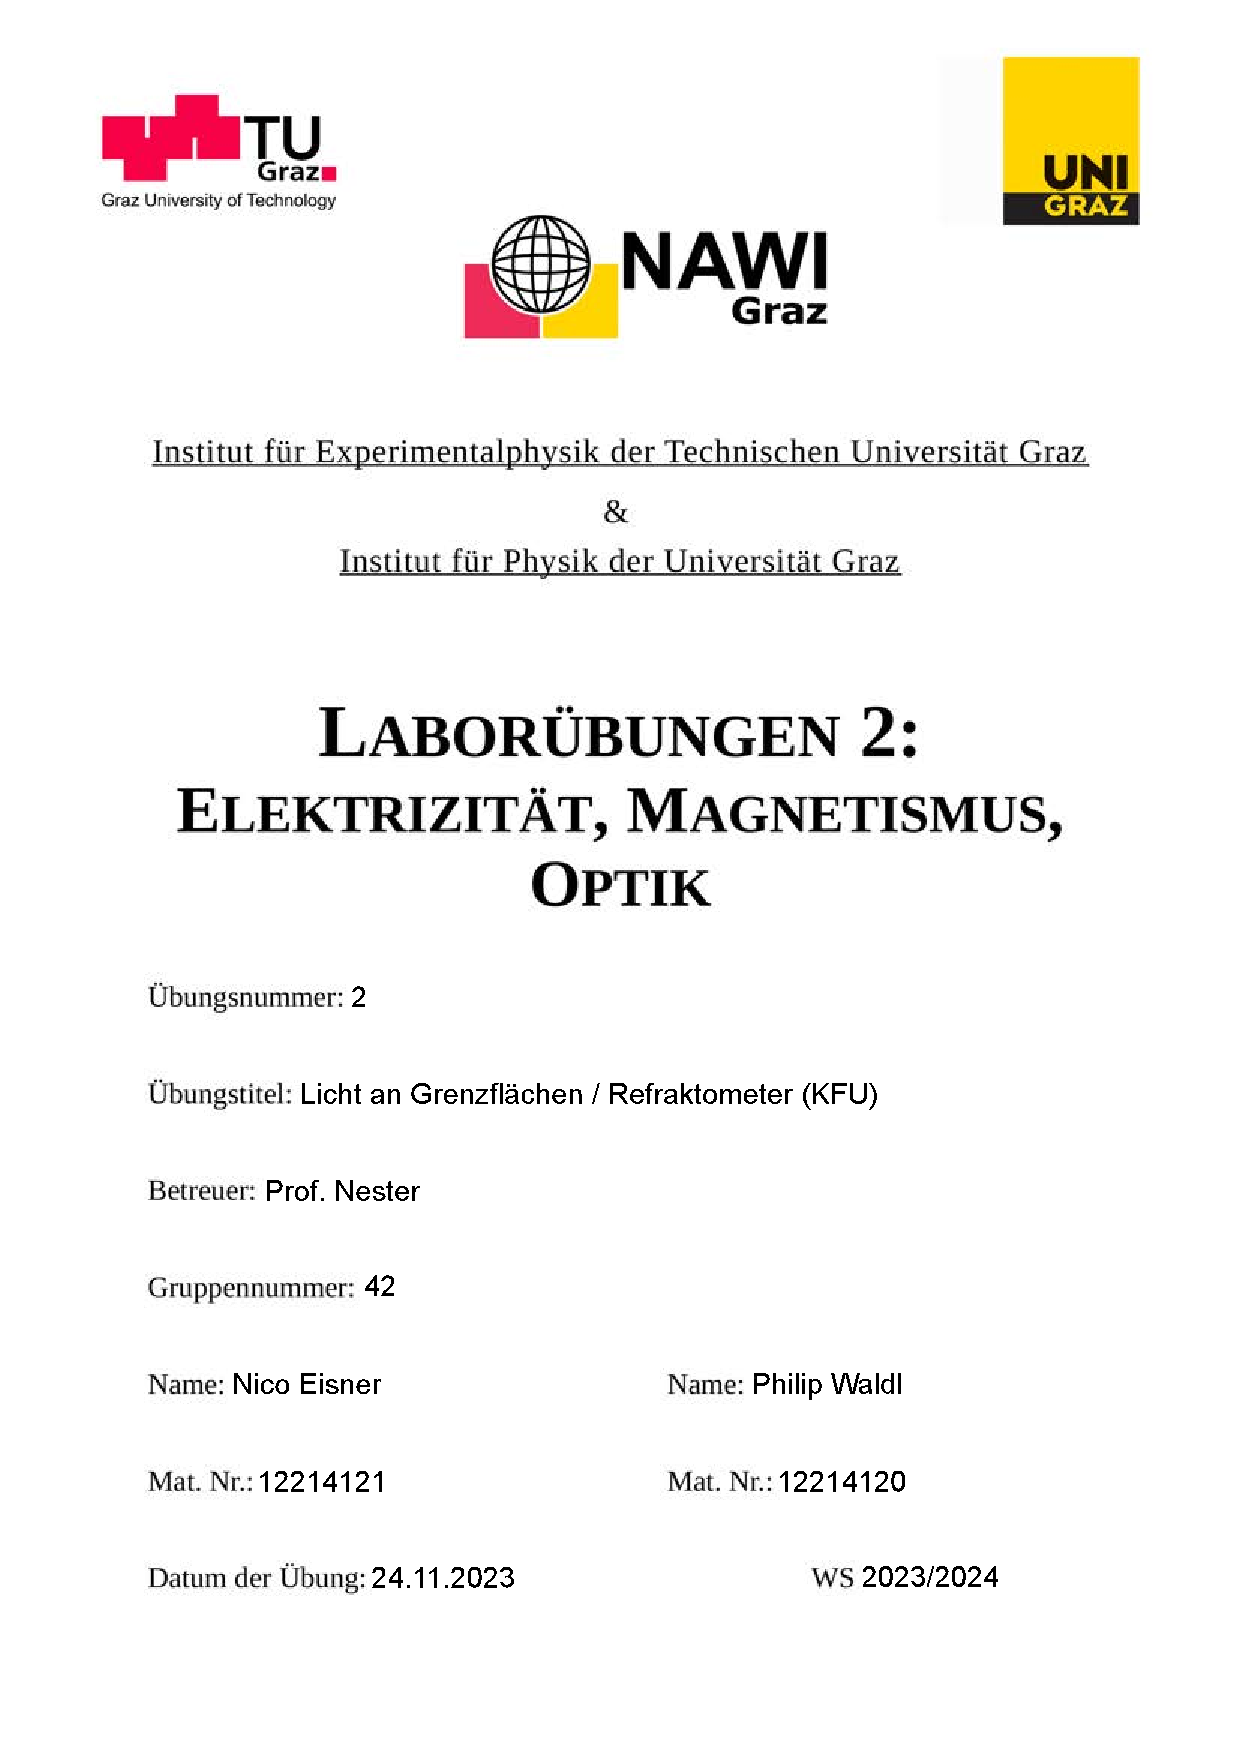
\includepdf[pages={1}]{../Deckblätter/Deckblatt_Refraktometer.pdf}

\tableofcontents
\newpage

\section{Aufgabenstellung} %jo beschreibn wos gmocht host ------------------------------
Das Experiment Licht an Grenzflächen / Refraktometer besteht aus drei Teilversuchen. 
\\
Im Ersten, wird mit einem Reflexions-Refraktometer an einer Grenzfläche zweier Medien das Reflexionsvermögen gemessen. 
Dabei ist die Messung von Medium 1 zu Medium 2 und umgekehrt durchzuführen. 
\\
Im zweiten Teilversuch wird das Brechungsgesetz bewiesen. 
\\
Im dritten Teilversuch werden mit einem Abbe-Refraktometer die Brechungsindizes zweier verschiedener Flüssigkeiten bestimmt, sowie die Menge an Zucker in einer Lösung. 
\\
\\
Alle Informationen und Methodiken wurden uns von der Technischen Universität bereitgestellt \cite{teachcenter2}. 

\section{Voraussetzungen \& Grundlagen} %Grundlagen erklären, Formeln mit erklärung
Um mit dem Experiment zu beginnen, gilt es erst einige Grundlagen zu kennen. 
\\
\\
Um das Reflexionsvermögen $R$ zu bestimmen, benötigt man die Detektorspannungen bei direktem Einfall des Laserstrahles $U_0$ sowie bei reflektiertem Einfall des Laserstrahles durch die Medien $U_R$. 
Wenn der Laserstrahl nicht auf den Detektor trifft, ist dennoch eine Spannung zu messen. Diese Spannung $U_D$ ist das Dunkelstromrauschen des Detektors und der Photostrom der Umgebungsbeleuchtung. 
\\
Um nun das Reflexionsvermögen $R$ zu berechnen, benötigt man die Intensität $I$ welche vom Detektor ausgebeben wird. 
Dabei ist die Refernzintensität 

\begin{equation}
    \label{eq:Refernzintensität}
    \centerline{$I_0 \varpropto U_0 - U_D$ \\ $\Delta I_0 = \vert \frac{\partial I_0}{\partial U_0} * \Delta U_0 \vert + \vert \frac{\partial I_0}{\partial U_D} * \Delta U_D \vert$}
\end{equation}

\noindent
und die Reflexionsintensität 

\begin{equation}
    \label{eq:Reflexionsintensität}
    \centerline{$I_R \varpropto U_R - U_D$ \\ $\Delta I_R = \vert \frac{\partial I_R}{\partial U_R} * \Delta U_R \vert + \vert \frac{\partial I_R}{\partial U_D} * \Delta U_D \vert$}
\end{equation}

\noindent 
Daraus lässt sich das Reflexionsvermögen $R$ mit Unsicherheit $\Delta R$ berechnen. 

\begin{equation}
    \label{eq:Reflexionsvermögen}
    \centerline{$R=\frac{I_R}{I_0}$ \\ $\Delta R = \vert \frac{\partial R}{\partial I_R} * \Delta I_R \vert + \vert \frac{\partial R}{\partial I_0} * \Delta I_0 \vert$}
\end{equation}

\noindent
Im Ersten Teil wird das Reflexionsvermögen bei einem p-Polarisierten und einen s-Polarisierten Laserstrahl gemessen. 
\\
Ein p-Polarisierter Laserstrahl ist parallel zur Einfallsebene polarisiert und ein s-Polarisierter senkrecht zur Einfallsebene. 
P-Polarisation lässt sich durch den Brewsterwinkel bestimmen. Dazu dreht man den Polarisator so lange, bis der reflektierte Strahl ab einen gewissen Winkel verschwindet. 
Um 90° verschoben ist der Laserstrahl s-Polarisiert.
\\
Der Brewsterwinkel ist jener Winkel, bei welchem ab einem bestimmten Einfallswinkel die Helligkeit im Minimum null ist \cite{Brewster}. 
Wird der Lichtstrahl so gebrochen, dass der Einfallswinkel einen Brechungswinkel von 90° zufolge hat, spricht man vom Grenzwinkel der Totalreflexion \cite{Grenzwinkel}. 


\begin{figure}[H]
    \centering
    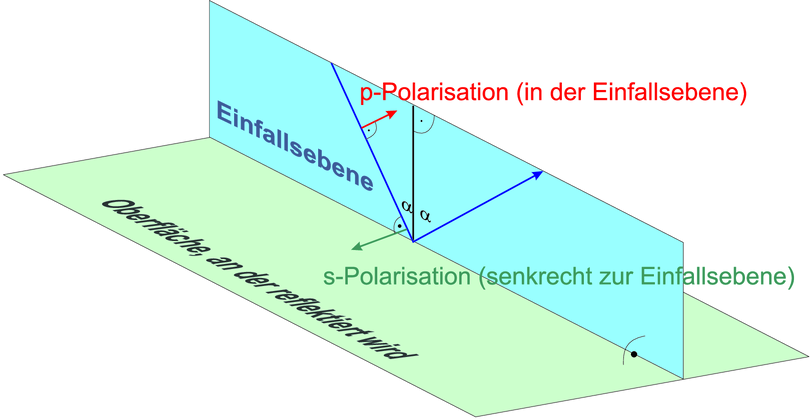
\includegraphics[width=0.6\linewidth]{nudes/sp pol.png}
    \caption{Darstellung eines p-Polarisierten und s-Polarisierten Lichtstrahles. \cite{Polarisation}}
    \label{fig:s-p-Polarisiert}
\end{figure}

\noindent
Um den Brechungswinkel $\beta$ zu bestimmen, benötigt man das Brechungsgesetz von Snellius. Dafür benötigt man die Brechungsindizes $n$ der Medien sowie den einfallenden Winkel $\alpha$. 

\begin{equation}
    \label{eq:Snellius}
    \centerline{$n_1 * sin(\alpha) = n_2 * sin(\beta)$}
\end{equation}

\noindent
Durch Umformen des Gesetzes lässt sich der Sinus von $\beta$ berechnen. Um den Winkel $\beta$ zu erhalten, wird der Wert nochmals in den Arcussinus eingesetzt. 

\begin{equation}
    \label{eq:Brechender Winkel}
    \centerline{$\beta = arcsin(\frac{n_1 * sin(\alpha)}{n_2})$ \\ $\Delta \beta = \vert \frac{\partial \beta}{\partial \alpha} * \Delta \alpha \vert + \vert \frac{\partial \beta}{\partial n_1} * \Delta n_1 \vert + \vert \frac{\partial \beta}{\partial n_2} * \Delta n_2 \vert$}
\end{equation}

\noindent
Für die Bestimmung der Brechungsindizes $n$ mit einem Abbe-Refraktometer benötigt man die im Okular abgelesene Werte des Brechungsindex $n_D$ und Brix sowie den Kompensatorwert. 
Mithilfe des Nomogrammes wird die mittlere Dispersion $n_F-n_C$ bestimmt. Dabei stehen die Buchstaben $D, F, C$ für die Fraunhofer Linien \cite{Fraunhofer}.  

\begin{figure}[H]
    \centering
    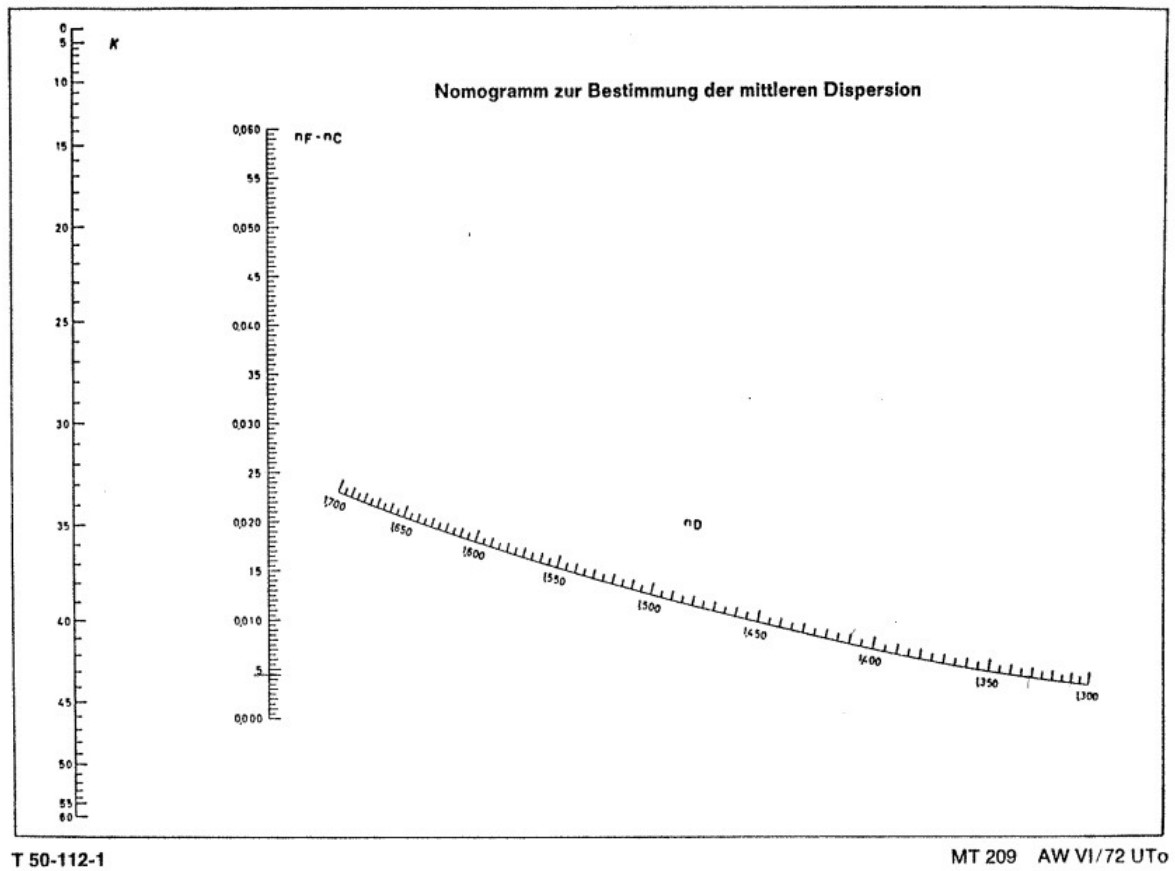
\includegraphics[width=0.6\linewidth]{nudes/nomogramm.jpg}
    \caption{Nomogramm zur bestimmung der mittleren Dispersion $n_F-n_C$. Entnommen aus Skript Fresnel Seite 14. \cite{teachcenter2}}
    \label{fig:nomogramm}
\end{figure}

\noindent
Desweiteren wird die Menge an gelöstem Zucker benötigt. Über die Skala Brix lässt sich diese bestimmen. 
Ein Grad Brix, oder ein Prozent Brix, entspricht dabei 1 Gramm Saccharose in 100 Gramm Lösung \cite{Brix}.

\section{Versuchsanordnung} %mit skizze kurz beschreiben ------------------------------
Der Versuch ist wiefolgt aufgebaut. 

\begin{figure}[H]
    \centering
    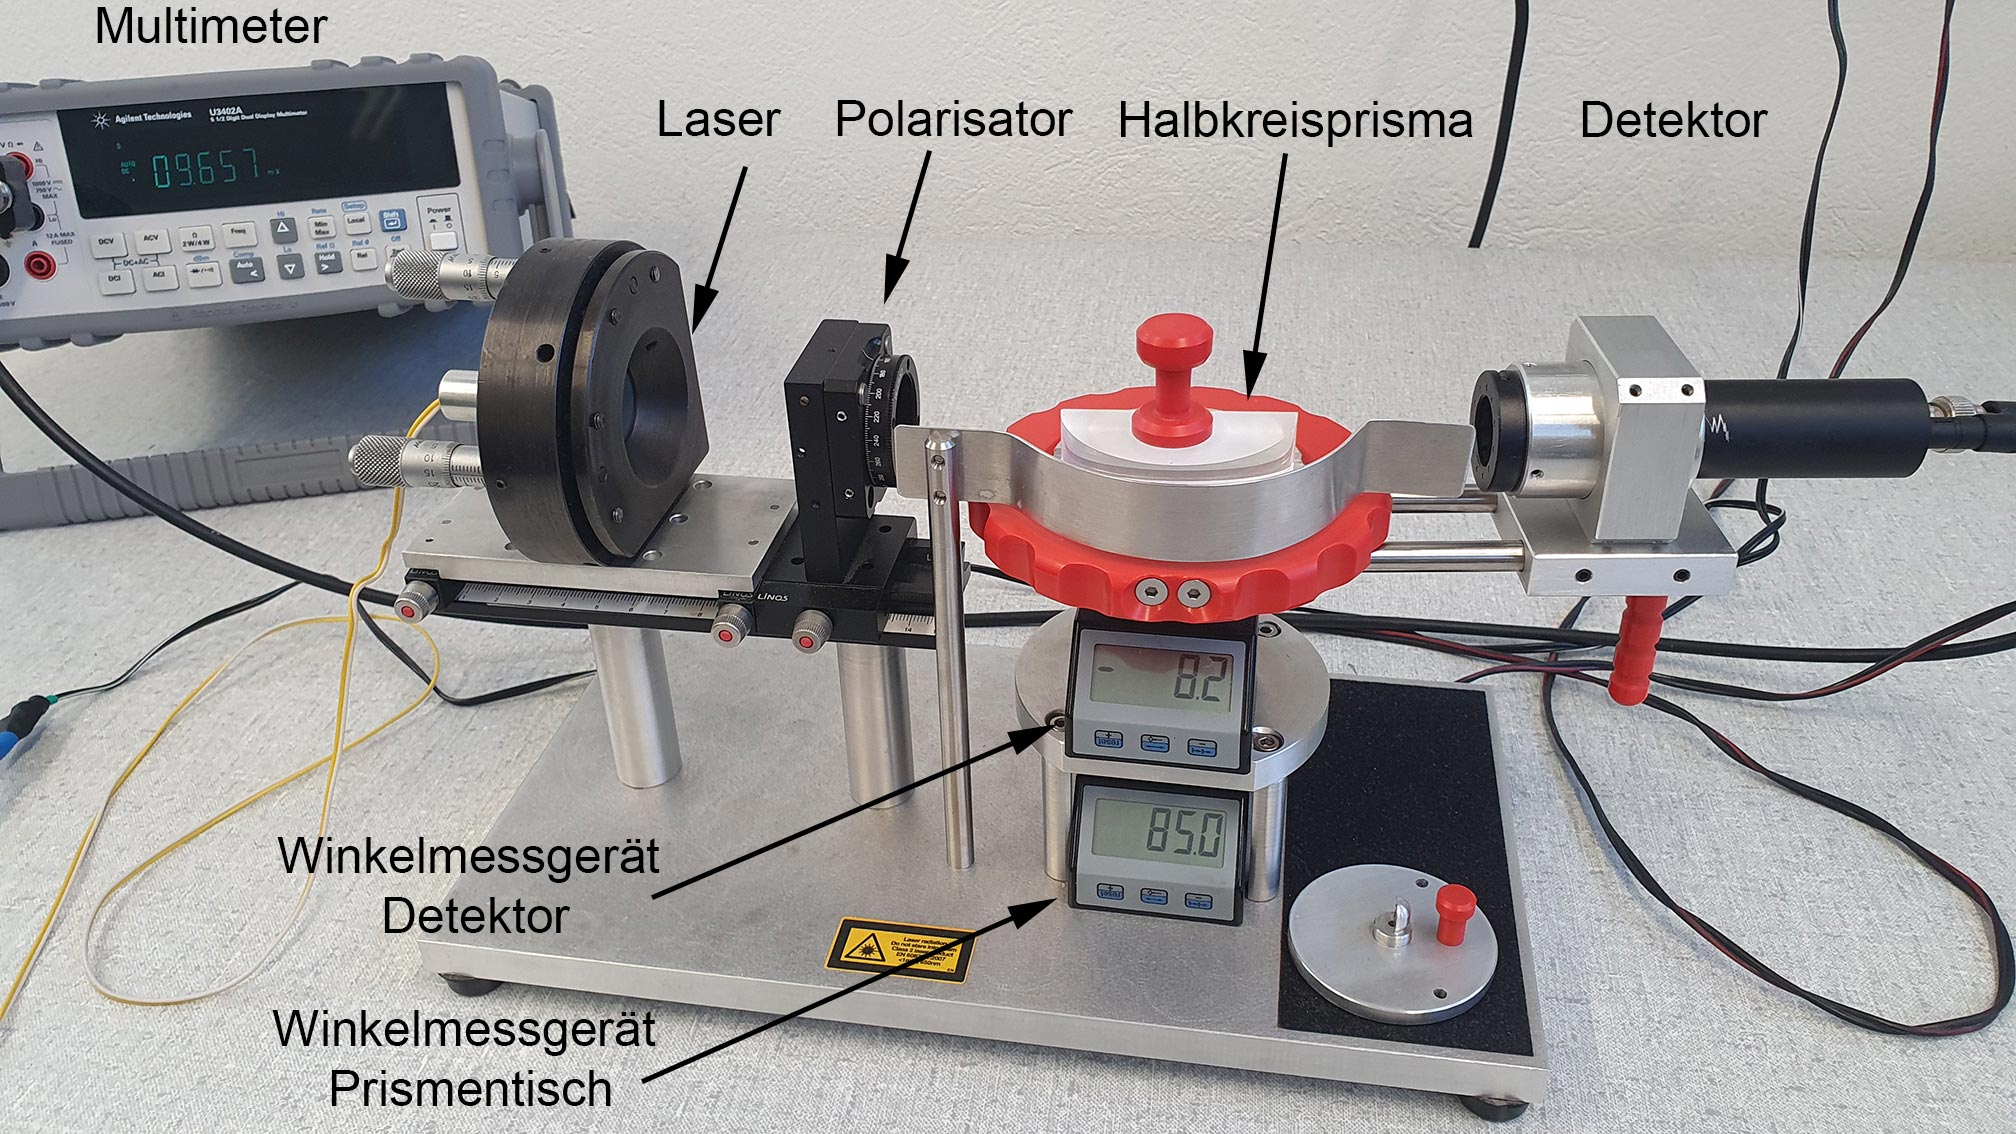
\includegraphics[width=0.7\linewidth]{nudes/Aufbau.jpg}
    \caption{Aufbau des Versuches Refexions-Refraktometer}
    \label{fig:aufbau}
\end{figure}

\noindent
Ein Laser sendet Lichtstrahlen durch einen Polarisator, welche auf einen Halbkreisprisma treffen. Dort werden die Lichtstrahlen gebrochen und es entsteht ein refkektierender Strahl und ein gebrochener Strahl. 
Dieser Strahl wird von einem Detektor gemessen und als Spannung am Multimeter dargestellt. 

\begin{figure}[H]
    \centering
    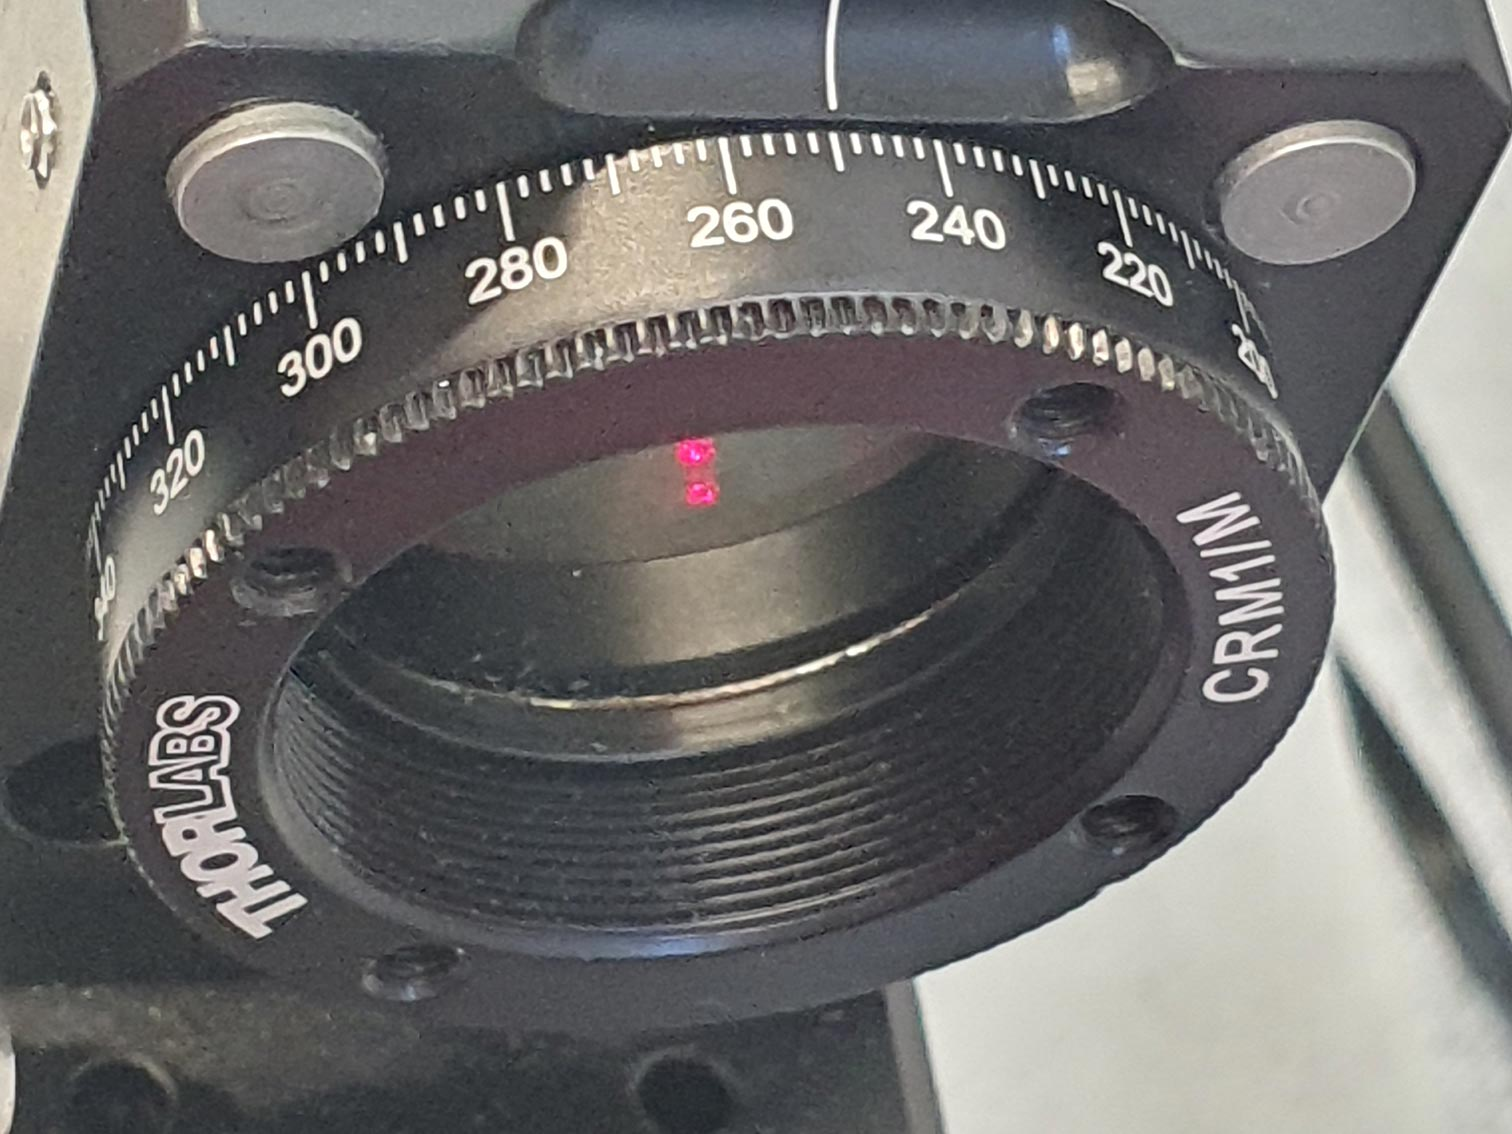
\includegraphics[width=0.4\linewidth]{nudes/Polarisator.jpg}
    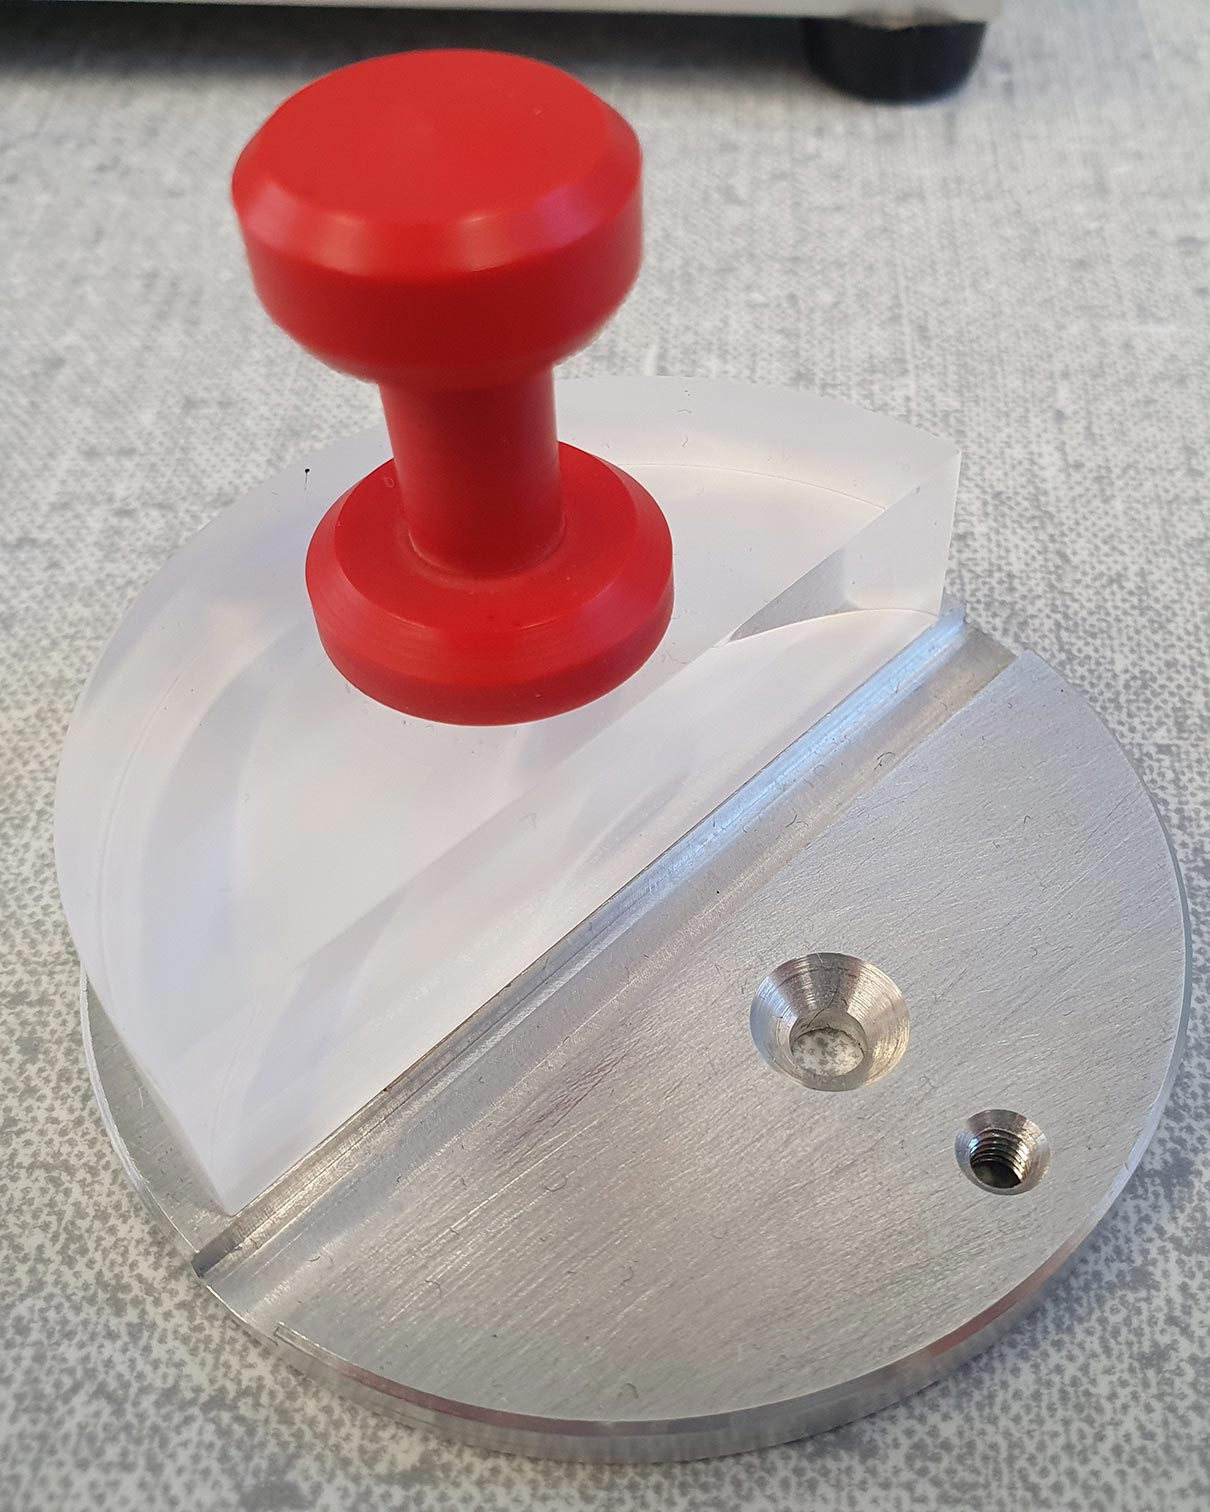
\includegraphics[width=0.4\linewidth]{nudes/halbkreisprisma.jpg}
    \caption{Polarisator mit Winkelskala (rechts) und Halbkreisprisma (links). }
    \label{fig:Polarisator und prisma}
\end{figure}

\noindent
Durch Drehen des Polarisators lässt sich der Lichtstrahl in p-Polarisiertes oder s-Polarisiertes Licht polarisieren. 
Dabei wird der Prisma gedreht und die Blende des Detektors wird geschlossen, um den Detektor genau auf den reflektierenden Strahl zu lenken. 
\\
\\
Bei dem Abbe-Refraktometer wird die zu bestimmende Flüssigkeit auf den Prisma gegeben. Durch die Beleuchtung mit weißem Licht kommt es zu einer Farbaufspaltung. 
Durch Ausgleichen dieser Aufspaltung mit Kompenstorprismen wird der Brechungsindex und Brix abgelesen. 

\begin{figure}[H]
    \centering
    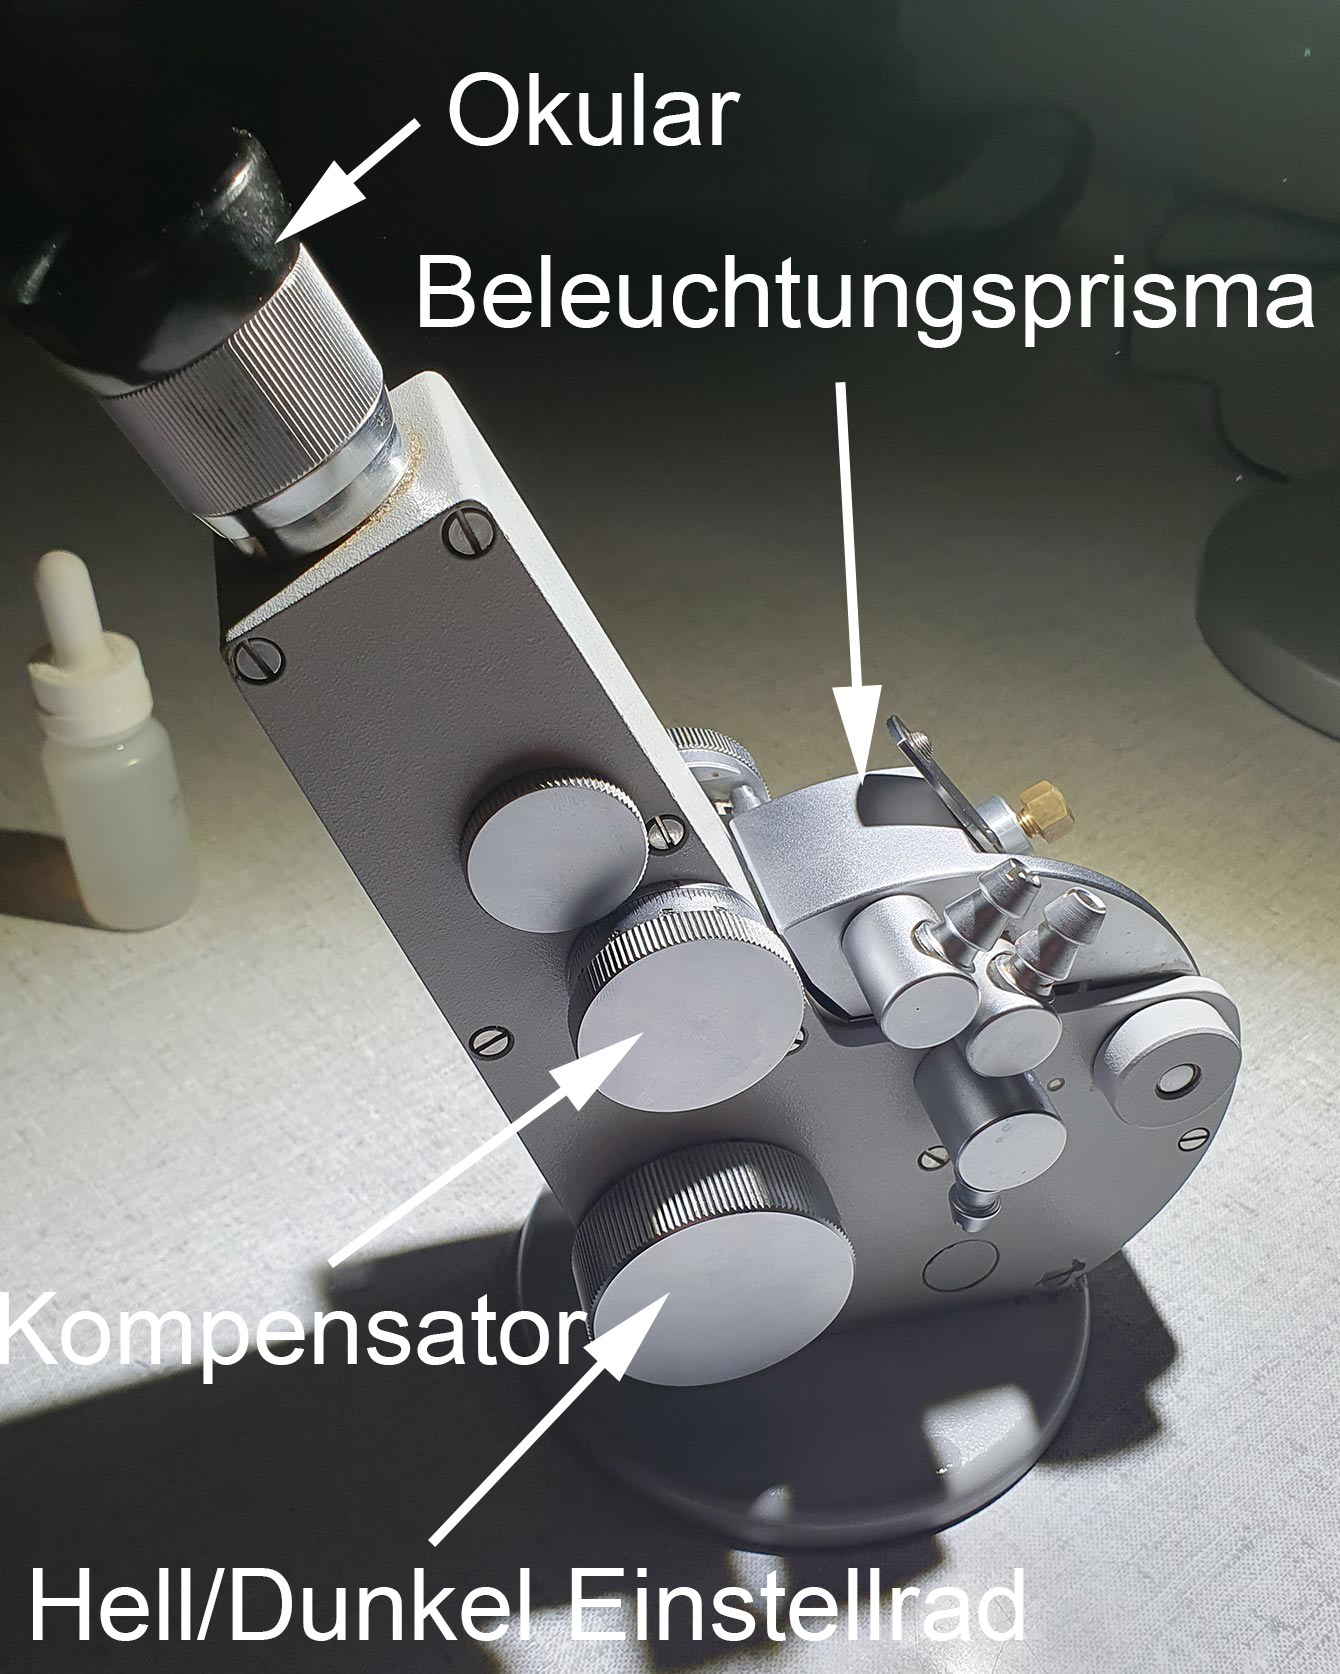
\includegraphics[width=0.4\linewidth]{nudes/abbe.jpg}
    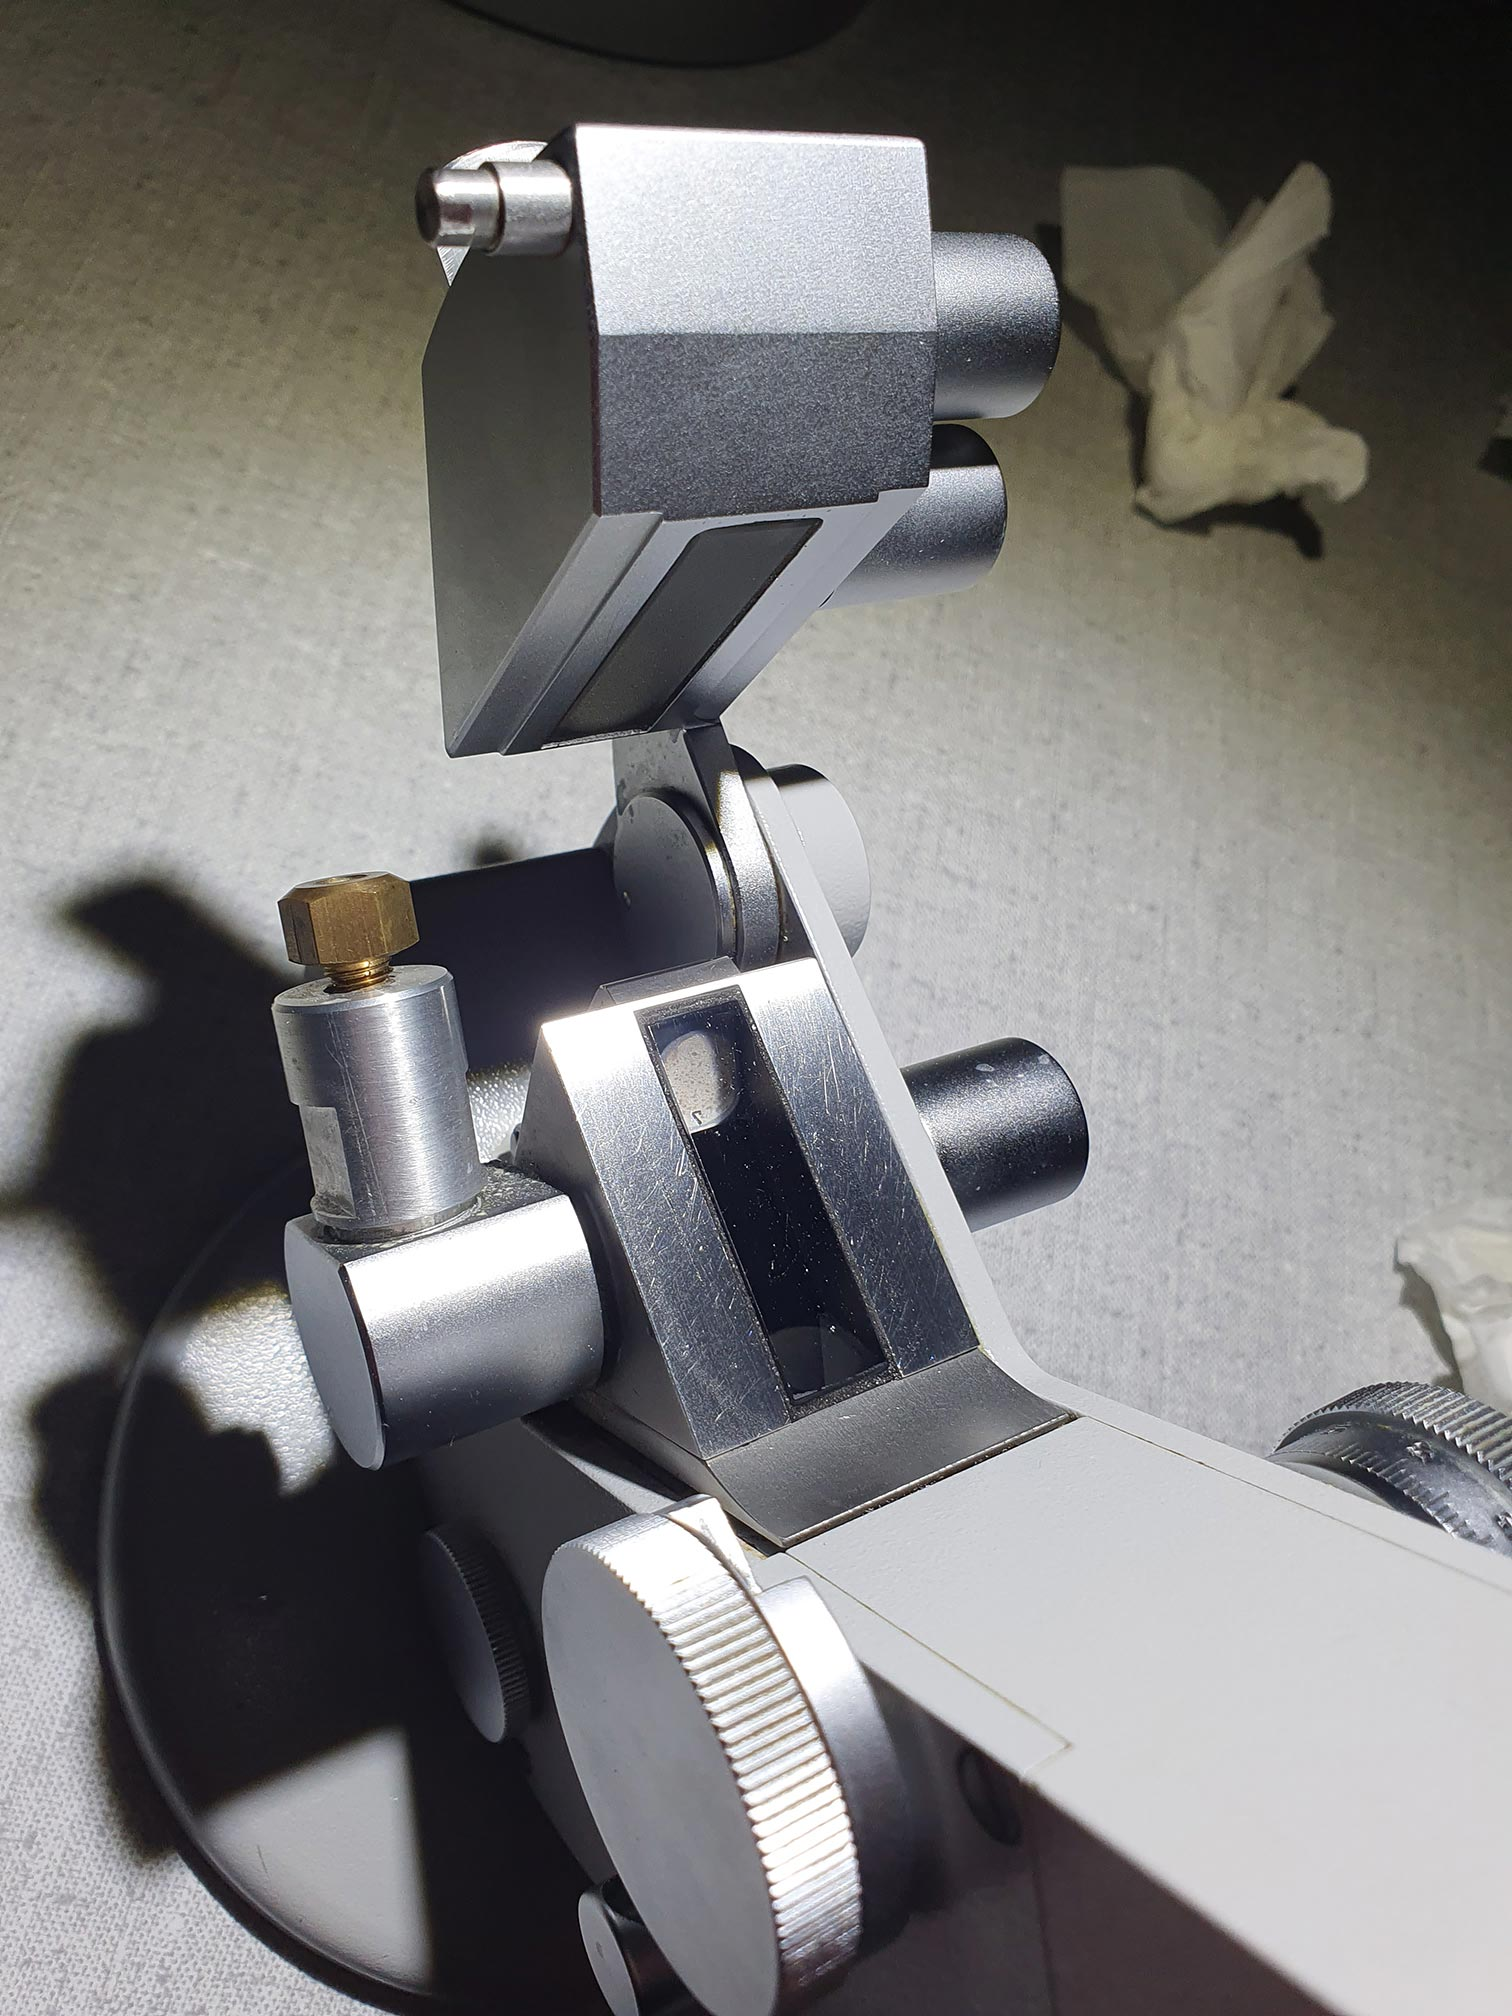
\includegraphics[width=0.4\linewidth]{nudes/abbe2.jpg}
    \caption{Aufbau des Versuches Abbe-Refraktometer (links). Beleuchtungsprisma ohne zu messender Flüssigkeit (rechts). }
    \label{fig:abbe}
\end{figure}



\section{Geräteliste} %jo holt a listn ------------------------------

    \begin{table}[H]
        \centering
        \caption{Im Versuch verwendete Geräte und Utensilien.}
        \label{tab:geraete}
        \begin{tabular}{| l | l | l |}
            \hline
            Gerät   & Gerätenummer  & Unsicherheit \\
            \hline
            Abbe-Refraktometer & {n.a} & {n.a} \\
            Reflexions-Refraktometer & {n.a} & {n.a} \\
            Laser & {n.a} & {n.a} \\
            Polarisator & Thorlabs CRM1/M & $\pm 2 deg. $ \\
            Halbkreisprisma & {n.a} & {n.a} \\
            Detektor & {n.a} & {n.a} \\
            Winkelmessgerät & {n.a} & $\pm 0.1 deg. $ \\
            Multimeter <120 mV & U3402A & $\pm 0.012 \% + 8 dig$ \cite{multimeter} \\
            Multimeter 120 - 1200 mV & U3402A & $\pm 0.012 \% + 5 dig$ \cite{multimeter} \\
            Wasser/Zucker Probe & {n.a} & {n.a}\\
            \hline
        \end{tabular}
    \end{table}


\section{Versuchsdurchführung \& Messergebnisse} %nachvollziehbar und klar dargestellt ------------------------------
Anmerkung. In den Tabellen ist ab ca. 120mV ein Sprung der Signifikanten Stellen zu beobachten. Dies liegt am Messgerätebereich, da dieser automatisch umschaltet, wie in der Geräteliste ersichtlich ist. 
\\
\\
Bevor die Messungen beginnen, gilt es die Winkelskalen einzustellen. Dazu schließt man die Blende komplett, entfernt den Halbkreisprisma und richtet den Detektor zentral auf den Laser. 
Das ist die null-Position. Der Prisma wir wieder eingesetzt und so eingestellt, dass der reflektierte Strahl wieder zum Laser zurückreflektiert wird. Das ist die null-Position des Prismas. 
Zur überprüfung wird der Prisma auf 45.0° gedreht und der Detektor auf 90.0°. Der reflektierte Strahl sollte genau auf den Detektor fallen. 
Dies tut er jedoch nur bei einem Winkel von 90.7°, was bedeutet, dass die Messung eine Winkelunsicherheit von $\Delta \varphi \pm 0.7 deg. $ hat. 
\\
\\
Im ersten Teil mit dem Reflextions-Refraktometer wird der reflektierte Srahl einer Luft-Glas Grenzschicht gemessen. 
Zuvor wird jedoch noch der Brewsterwinkel bestimmt. Bei entfernten Prisma wird einmal für p-Polarisiertes (110°) und einmal für s-Polarisiertes (200°) Licht die Referenzspannung $U_0$ gemessen. 
Der Prisma wird wieder eingesetzt und der Versuch wird wie in Abbildung \ref{fig:aufbau} aufgebaut. Durch schrittweises Drehen des Prismentisches wird der Einfallswinkel $\varphi_{Ein}$ verändert. Der Detektorwinkel $\varphi_D$ wird durch Drehen des Detektors bestimmt. Um genau die Mitte des Detektors zu treffen, 
wir die Blende geschlossen und der reflektierte Strahl auf die Mitte der Blende gerrichtet. Bei geöffneter Blende wird anschließend die reflektierte Spannung $U_R$ für einmal p-Polarisiertes und einmal für s-Polarisiertes Licht gemessen. 
Durch verdecken des Lasers wird die Detektorspannung $U_D$ gemessen. Dies wird insgesamt 15 mal wiederholt. 

\begin{table}[H]
    \centering
    \caption{Messergebnisse für eine Luft-Glas Grenzfläche bei p-Polarisiertem Licht. }
    \label{tab:mess luft glas p-pol}
    \begin{tabular}{| l | l | l | l | l | l |}
        \hline
        Nr. & $U_0 \pm 0.15 $ / mV & $U_D \pm 0.009$ / mV & $U_{R}$ / mV & $\varphi_{Ein} \pm 0.7$ / deg. & $\varphi_D \pm 0.7$ / deg.  \\
        \hline
        1  & 826.32 & -5.047 & 29.097 $\pm$ 0.012 & 15.0 & -147.8 \\
        2  & 826.32 & -5.184 & 15.378 $\pm$ 0.010 & 20.0 & -139.2 \\
        3  & 826.32 & -5.396 & 13.262 $\pm$ 0.010 & 25.0 & -128.0 \\
        4  & 826.32 & -5.594 & 10.798 $\pm$ 0.010 & 30.0 & -119.7 \\
        5  & 826.32 & -5.619 & 7.032  $\pm$ 0.009 & 35.0 & -109.4 \\
        6  & 826.32 & -5.863 & 3.184  $\pm$ 0.009 & 40.0 & -99.2  \\
        7  & 826.32 & -5.934 & -1.239 $\pm$ 0.008 & 45.0 & -87.9  \\
        8  & 826.32 & -5.932 & -4.141 $\pm$ 0.008 & 50.0 & -79.1  \\
        9  & 826.32 & -5.972 & -5.824 $\pm$ 0.008 & 55.0 & -68.5  \\
        10 & 826.32 & -5.962 & -4.574 $\pm$ 0.008 & 60.0 & -60.2  \\
        11 & 826.32 & -5.954 & 4.178  $\pm$ 0.009 & 65.0 & -49.8  \\
        12 & 826.32 & -5.905 & 26.375 $\pm$ 0.012 & 70.0 & -39.4  \\
        13 & 826.32 & -5.874 & 82.346 $\pm$ 0.018 & 75.0 & -28.7  \\
        14 & 826.32 & -5.874 & 183.75 $\pm$ 0.07  & 80.0 & -19.2  \\
        15 & 826.32 & -5.852 & 419.78 $\pm$ 0.10  & 85.0 & -8.2   \\
        \hline
    \end{tabular}
\end{table}

\begin{table}[H]
    \centering
    \caption{Messergebnisse für eine Luft-Glas Grenzfläche bei s-Polarisiertem Licht. }
    \label{tab:mess luft glas s-pol}
    \begin{tabular}{| l | l | l | l | l | l |}
        \hline
        Nr. & $U_0 \pm 0.12 $ / mV & $U_D \pm 0.009$ / mV & $U_{R}$ / mV & $\varphi_{Ein} \pm 0.7$ / deg. & $\varphi_D \pm 0.7$ / deg.  \\
        \hline
        1  & 555.54 & -5.047 & 14.638  $\pm$ 0.010 & 15.0 & -147.8 \\
        2  & 555.54 & -5.184 & 16.944  $\pm$ 0.011 & 20.0 & -139.2 \\
        3  & 555.54 & -5.396 & 17.215  $\pm$ 0.011 & 25.0 & -128.0 \\
        4  & 555.54 & -5.594 & 18.226  $\pm$ 0.011 & 30.0 & -119.7 \\
        5  & 555.54 & -5.619 & 22.588  $\pm$ 0.011 & 35.0 & -109.4 \\
        6  & 555.54 & -5.863 & 27.110  $\pm$ 0.012 & 40.0 & -99.2  \\
        7  & 555.54 & -5.934 & 37.612  $\pm$ 0.013 & 45.0 & -87.9  \\
        8  & 555.54 & -5.932 & 46.118  $\pm$ 0.014 & 50.0 & -79.1  \\
        9  & 555.54 & -5.972 & 58.697  $\pm$ 0.016 & 55.0 & -68.5  \\
        10 & 555.54 & -5.962 & 78.027  $\pm$ 0.018 & 60.0 & -60.2  \\
        11 & 555.54 & -5.954 & 100.634 $\pm$ 0.020 & 65.0 & -49.8  \\
        12 & 555.54 & -5.905 & 136.88  $\pm$ 0.07 & 70.0 & -39.4  \\
        13 & 555.54 & -5.874 & 208.06  $\pm$ 0.08 & 75.0 & -28.7  \\
        14 & 555.54 & -5.874 & 280.71  $\pm$ 0.09 & 80.0 & -19.2  \\
        15 & 555.54 & -5.852 & 392.42  $\pm$ 0.10 & 85.0 & -8.2   \\
        \hline
    \end{tabular}
\end{table}

\noindent
Für eine Glas-Luft Grenzfläche wird der Versuch wiederholt. Dazu dreht man den Prismentisch auf 180°, dreht den Prisma um und somit hat man eine neue null-Position auf der Winkelskala. 

\begin{table}[H]
    \centering
    \caption{Messergebnisse für eine Glas-Luft Grenzfläche bei p-Polarisiertem Licht. }
    \label{tab:mess glas luft p-pol}
    \begin{tabular}{| l | l | l | l | l | l |}
        \hline
        Nr. & $U_0 \pm 0.15 $ / mV & $U_D \pm 0.009$ / mV & $U_{R}$ / mV & $\varphi_{Ein} \pm 0.7$ / deg. & $\varphi_D \pm 0.7$ / deg.  \\
        \hline
        1  & 826.32 & -5.425 & 10.268 $\pm$ 0.010 & 15.0 & -148.6 \\
        2  & 826.32 & -5.359 & 6.894  $\pm$ 0.009 & 20.0 & -139.1 \\
        3  & 826.32 & -5.511 & 1.776  $\pm$ 0.009 & 25.0 & -128.1 \\
        4  & 826.32 & -5.543 & -2.431 $\pm$ 0.008 & 30.0 & -120.5 \\
        5  & 826.32 & -5.719 & -0.478 $\pm$ 0.008 & 35.0 & -110.0 \\
        6  & 826.32 & -5.789 & 36.692 $\pm$ 0.013 & 40.0 & -99.8  \\
        7  & 826.32 & -5.936 & 519.59 $\pm$ 0.12  & 45.0 & -88.7  \\
        8  & 826.32 & -5.908 & 510.97 $\pm$ 0.12  & 55.0 & -68.4  \\
        10 & 826.32 & -5.955 & 557.28 $\pm$ 0.12  & 60.0 & -60.4  \\
        11 & 826.32 & -5.963 & 589.87 $\pm$ 0.13  & 65.0 & -50.1  \\
        12 & 826.32 & -5.915 & 638.36 $\pm$ 0.13  & 70.0 & -39.8  \\
        13 & 826.32 & -5.832 & 668.14 $\pm$ 0.14  & 75.0 & -29.1  \\
        14 & 826.32 & -5.817 & 688.48 $\pm$ 0.14  & 80.0 & -19.4  \\
        15 & 826.32 & -5.879 & 700.82 $\pm$ 0.14  & 85.0 & -8.5   \\
        \hline
    \end{tabular}
\end{table}

\begin{table}[H]
    \centering
    \caption{Messergebnisse für eine Glas-Luft Grenzfläche bei s-Polarisiertem Licht. }
    \label{tab:mess glas luft s-pol}
    \begin{tabular}{| l | l | l | l | l | l |}
        \hline
        Nr. & $U_0 \pm 0.12 $ / mV & $U_D \pm 0.009$ / mV & $U_{R}$ / mV & $\varphi_{Ein} \pm 0.7$ / deg. & $\varphi_D \pm 0.7$ / deg.  \\
        \hline
        1  & 555.54 & -5.425 & 12.193  $\pm$ 0.010 & 15.0  & -148.6 \\
        2  & 555.54 & -5.359 & 16.648  $\pm$ 0.010 & 20.0  & -139.1 \\
        3  & 555.54 & -5.511 & 21.414  $\pm$ 0.011 & 25.0  & -128.1 \\
        4  & 555.54 & -5.543 & 29.556  $\pm$ 0.012 & 30.0  & -120.5 \\
        5  & 555.54 & -5.719 & 55.858  $\pm$ 0.015 & 35.0  & -110.0 \\
        6  & 555.54 & -5.789 & 119.634 $\pm$ 0.023 & 40.0  & -99.8  \\
        7  & 555.54 & -5.936 & 367.57  $\pm$ 0.10  & 45.0  & -88.7  \\
        8  & 555.54 & -5.908 & 360.52  $\pm$ 0.10  & 50.0  & -79.5  \\
        9  & 555.54 & -5.915 & 346.67  $\pm$ 0.10  & 55.0  & -68.4  \\
        10 & 555.54 & -5.955 & 378.43  $\pm$ 0.10  & 60.0  & -60.4  \\
        11 & 555.54 & -5.963 & 388.25  $\pm$ 0.10  & 65.0 & -50.1  \\
        12 & 555.54 & -5.915 & 409.67  $\pm$ 0.10  & 70.0 & -39.8  \\
        13 & 555.54 & -5.832 & 427.86  $\pm$ 0.11  & 75.0 & -29.1  \\
        14 & 555.54 & -5.817 & 447.67  $\pm$ 0.11  & 80.0 & -19.4  \\
        15 & 555.54 & -5.879 & 482.37  $\pm$ 0.11  & 85.0 & -8.5   \\
        \hline
    \end{tabular}
\end{table}

\noindent
Im dritten Teil des Experimentes mit dem Reflexions-Refraktometer wird der brechende-Winkel einer Luft-Glas Grenzfläche bestimmt. 
Dazu wird der Versuch erneut wie in Abbildung \ref{fig:aufbau} aufgebaut. Durch drehen des Prisma in die andere Richtung ist der gebrochene Strahl erkennbar. 
Der Detektor wird auf diesen ausgerichtet und die Winkel werden insgesamt 10 mal gemessen. 

\begin{table}[H]
    \centering
    \caption{Einfallswinkel $\varphi_{Ein}$ und brechender Winkel $\varphi_D$ einer Luft-Glas Grenzfläche. }
    \label{tab:brechender Winkel}
    \begin{tabular}{| l | l | l |}
        \hline
        Nr. &  $\varphi_{Ein} \pm 0.7$ / deg. & $\varphi_D \pm 0.7$ / deg.  \\
        \hline
        1   & 20.0  & -6.8  \\
        2   & 25.0  & -8.1  \\
        3   & 30.0  & -10.0 \\
        4   & 35.0  & -11.3 \\
        5   & 40.0  & -13.7 \\
        6   & 45.0  & -15.7 \\
        7   & 50.0  & -19.2 \\
        8   & 55.0  & -21.4 \\
        9   & 60.0  & -24.2 \\
        10  & 65.0  & -27.0 \\
        \hline
    \end{tabular}
\end{table}

\noindent
Im letzten Teil des Experimentes werden mithilfe eines Abbe-Refraktometers die Brechungsindizes von Flüssigkeiten bestimmt. 
Dazu Reinigt man zuvor den Beleuchtungsprisma (Abb. \ref{fig:abbe}) mit destilierten Wasser, um sicher zu gehen, dass vom vorherigen Versuch keine Rückstände vorhanden sind. 
Man gibt einige Tropfen destilliertes Wasser auf den Messprisma und klappt den Beleuchtungsprisma zu. Durch drehen des Einstellknopfes (Abb. \ref{fig:abbe}) wird die Hell-Dunkel Grenze auf das Fadenkreuz ausgerichtet. 
Mit dem Kompensatorknopf wird die Farbaufspaltung korrigiert. Im Okular lässt sich der Brechungsindex $n_D$ sowie die Brix ablesen. Am Kompensatorknopf wird der Wert abgelesen. 
Dies wird für eine Zuckerlösung wiederholt. Die Unsicherheiten ergeben sich aus der Ableseunsicherheit. 

\begin{table}[H]
    \centering
    \caption{Brechungsindizes $n_D$, Brix und Kompensatorwert verschiedener Proben. }
    \label{tab:abbe werte}
    \begin{tabular}{| l | l | l | l |}
        \hline
        Typ &  $n_D \pm 0.0005$ /  & $Brix \pm 0.5$ / \% & Kompensatorwert $\pm 0.5$ / \\
        \hline
        Wasser   & 1.3335  & 0.5 & 43  \\
        Zuckerlösung & 1.3755  & 27.0  & 42  \\
        \hline
    \end{tabular}
\end{table}

\begin{figure}[H]
    \centering
    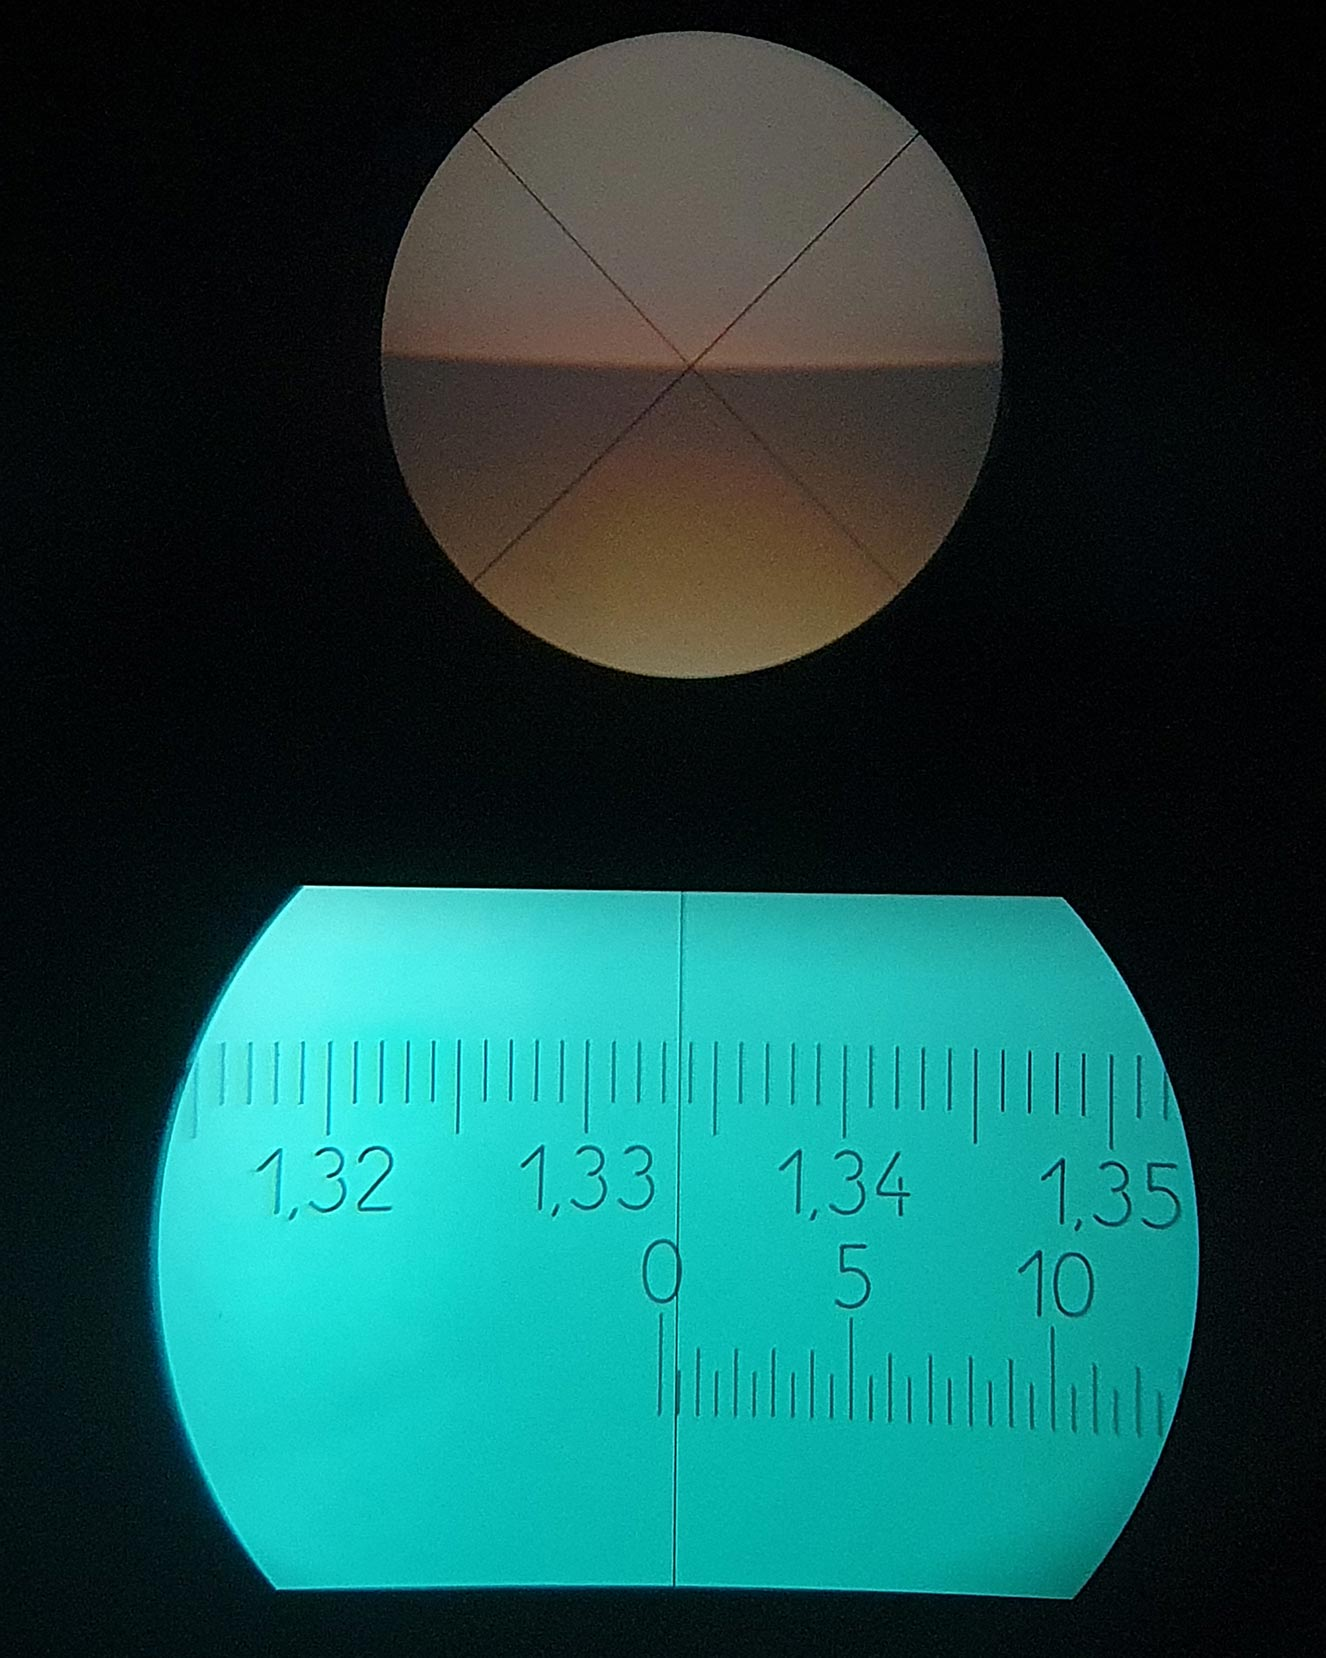
\includegraphics[width=0.4\linewidth]{nudes/wasser okular.jpg}
    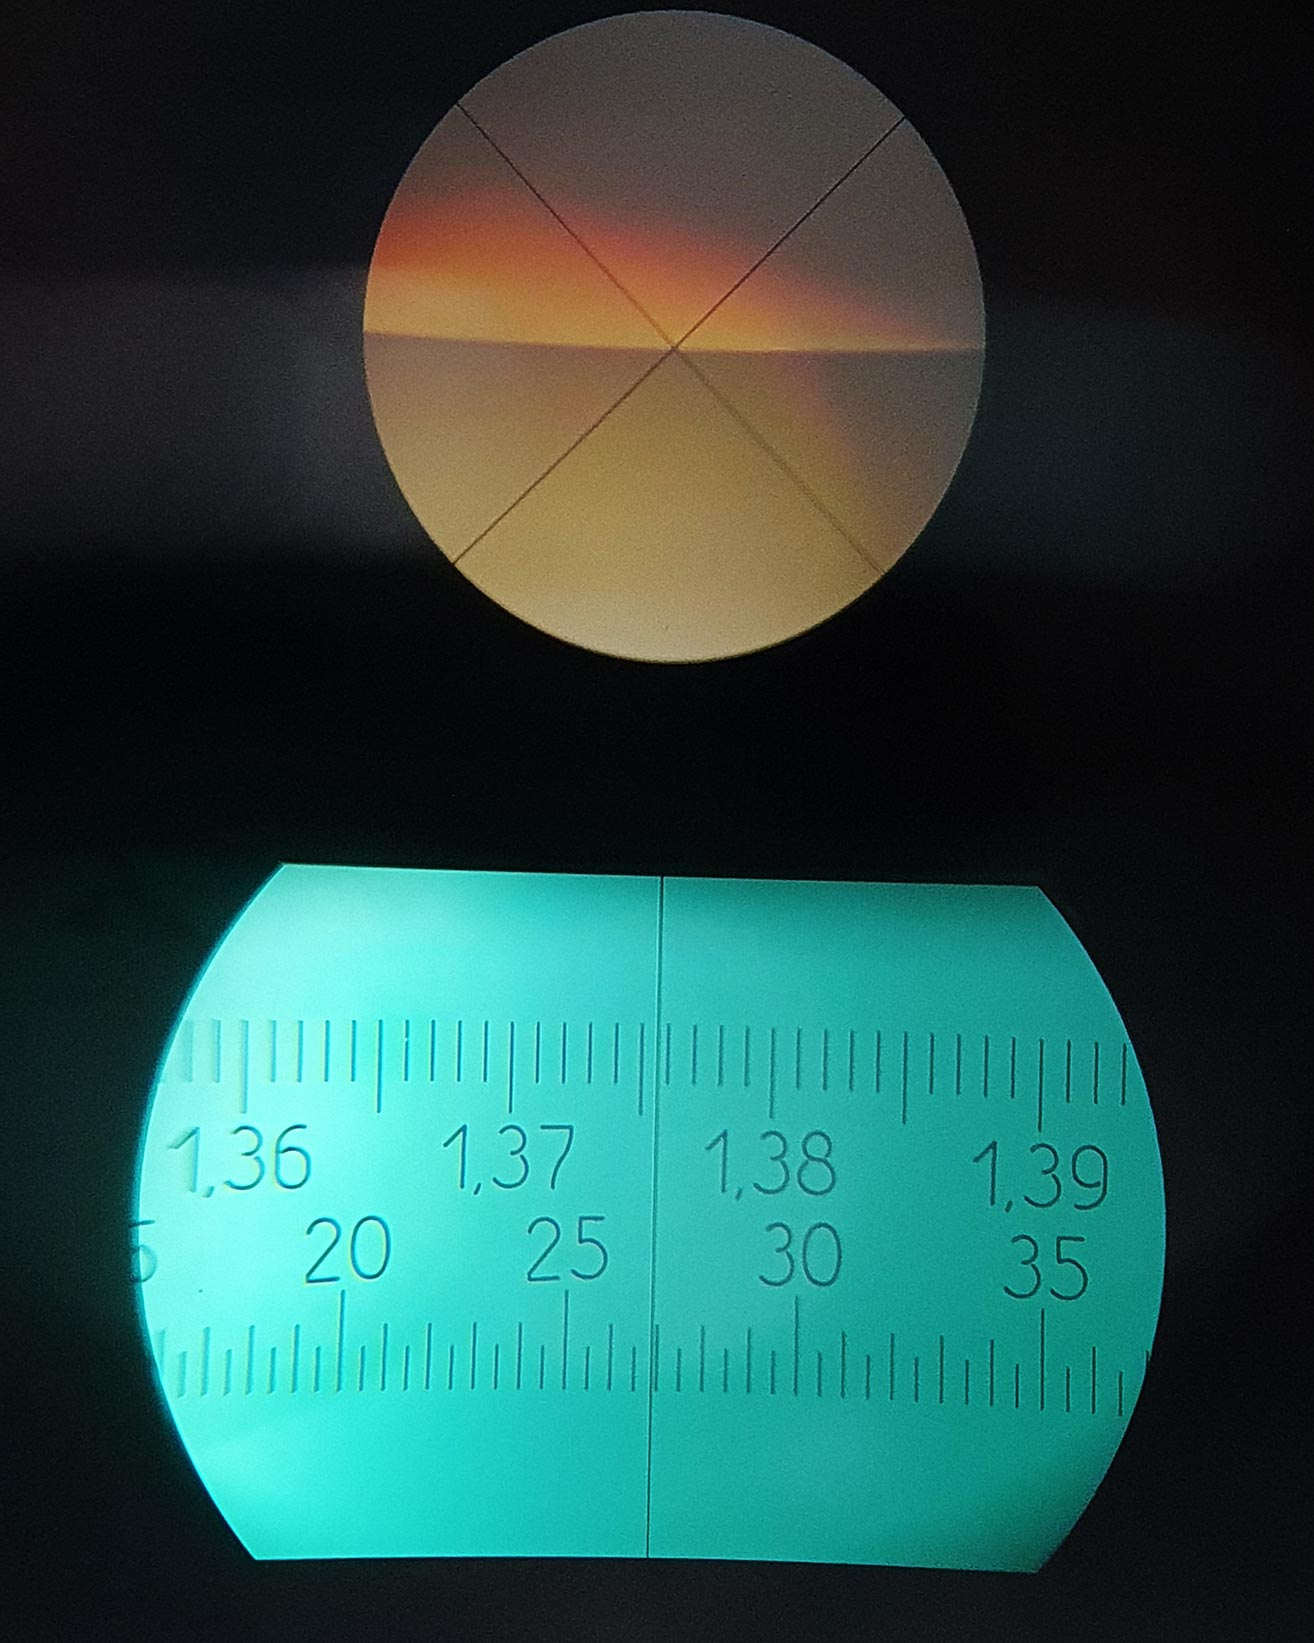
\includegraphics[width=0.4\linewidth]{nudes/zucker okular.jpg}
    \caption{Blick des Okulares. Brechungsindex des destillierten Wassers (links) und der Zuckerlösung (rechts). }
    \label{fig:zucker wasser}
\end{figure}

\section{Auswertung und Unsicherheitsanalyse} %Nicht nur zahlen angeben ------------------------------
In der Auswertung werden zur erhöhten Genauigkeit durchgehend ungerundete Werte bis zu den Endergebnissen verwendet und nur zur Darstellung gerundet. \\
Zur Berechnung der Unsicherheiten wird, wenn nicht anders angegeben, die Größtunsicherheitsmethode verwendet.
\\
\\
Für die Werte aus den Tabellen \ref{tab:mess luft glas p-pol} und \ref{tab:mess luft glas s-pol} wird das Reflexionsvermögen $R$ berechnet. 
Mit der Formel \ref{eq:Reflexionsvermögen} für das Reflexionsvermögen $R$ und den Intensitäten $I_0$ und $I_R$ (Formeln \ref{eq:Refernzintensität}, \ref{eq:Reflexionsintensität}) kommt man auf die folgenden Werte. 

\begin{table}[H]
    \centering
    \caption{Reflexionsvermögen $R$ sowie Refernzintensität $I_0$ und Reflexionsintensität $I_R$ für eine Luft-Glas Grenzfläche bei p-Polarisiertem und s-Polarisierten Licht.}
    \label{tab:reflexionsvermögen luft glas}
    \begin{tabular}{| l | l | l | l | l | l | l |}
        \hline
        Nr. & $I_{0_p} \pm 9$/mV & $I_{R_p}$ / mV & $R_p$ /  & $I_{0_s} \pm 6$/mV & $I_{R_s}$ / mV & $R_s$ / \\
        \hline
        1  & 832  & 34.2  $\pm$ 0.4     & 0.0411    $\pm$ 0.0008    & 561 & 19.7  $\pm$ 0.2    & 0.0352  $\pm$ 0.0007    \\
        2  & 832  & 20.6  $\pm$ 0.2     & 0.0248    $\pm$ 0.0005    & 561 & 22.2  $\pm$ 0.3    & 0.0395  $\pm$ 0.0008    \\
        3  & 832  & 18.66 $\pm$ 0.18    & 0.0225    $\pm$ 0.0005    & 561 & 22.7  $\pm$ 0.3    & 0.0404  $\pm$ 0.0008    \\
        4  & 832  & 16.40 $\pm$ 0.16    & 0.0198    $\pm$ 0.0004    & 562 & 23.9  $\pm$ 0.3    & 0.0425  $\pm$ 0.0009    \\
        5  & 832  & 12.66 $\pm$ 0.12    & 0.0153    $\pm$ 0.0003    & 562 & 28.3  $\pm$ 0.3    & 0.0503  $\pm$ 0.0010    \\
        6  & 833  & 9.05  $\pm$ 0.09    & 0.0109    $\pm$ 0.0003    & 562 & 33.0  $\pm$ 0.4    & 0.0588  $\pm$ 0.0012    \\
        7  & 833  & 4.70  $\pm$ 0.04    & 0.00565   $\pm$ 0.00010   & 562 & 43.6  $\pm$ 0.5    & 0.0776  $\pm$ 0.0016    \\
        8  & 833  & 1.791 $\pm$ 0.012   & 0.00216   $\pm$ 0.00004   & 562 & 52.1  $\pm$ 0.5    & 0.0928  $\pm$ 0.0019    \\
        9  & 833  & 0.148 $\pm$ 0.005   & 0.000178  $\pm$ 0.000004  & 562 & 64.7  $\pm$ 0.7    & 0.116   $\pm$ 0.003     \\
        10 & 833  & 1.388 $\pm$ 0.007   & 0.00167   $\pm$ 0.00003   & 562 & 84.0  $\pm$ 0.9    & 0.150   $\pm$ 0.004     \\
        11 & 833  & 10.14 $\pm$ 0.10    & 0.0122    $\pm$ 0.0003    & 562 & 107   $\pm$ 2      & 0.190   $\pm$ 0.004     \\
        12 & 833  & 32.3  $\pm$ 0.4     & 0.0389    $\pm$ 0.0008    & 562 & 143   $\pm$ 2      & 0.255   $\pm$ 0.006     \\
        13 & 833  & 88.3  $\pm$ 0.9     & 0.107     $\pm$ 0.003     & 562 & 215   $\pm$ 3      & 0.382   $\pm$ 0.009     \\
        14 & 833  & 190   $\pm$ 3       & 0.228     $\pm$ 0.005     & 562 & 287   $\pm$ 4      & 0.511   $\pm$ 0.011     \\
        15 & 833  & 426   $\pm$ 5       & 0.512     $\pm$ 0.011     & 562 & 399   $\pm$ 5      & 0.710   $\pm$ 0.015     \\
        \hline
    \end{tabular}
\end{table}


\begin{table}[H]
    \centering
    \caption{Reflexionsvermögen $R$ sowie Refernzintensität $I_0$ und Reflexionsintensität $I_R$ für eine Glas-Luft Grenzfläche bei p-Polarisiertem und s-Polarisierten Licht.}
    \label{tab:reflexionsvermögen glas luft}
    \begin{tabular}{| l | l | l | l | l | l | l |}
        \hline
        Nr. & $I_{0_p} \pm 9$/mV & $I_{R_p}$ / mV & $R_p$ /  & $I_{0_s} \pm 6$/mV & $I_{R_s}$ / mV & $R_s$ / \\
        \hline
        1  & 832  & 15.70 $\pm$ 0.15    & 0.0189      $\pm$ 0.0004     & 561 & 17.62   $\pm$ 0.17  & 0.0315  $\pm$ 0.0007 \\
        2  & 832  & 12.26 $\pm$ 0.12    & 0.0148      $\pm$ 0.0003     & 561 & 22.1    $\pm$ 0.3   & 0.0393  $\pm$ 0.0008 \\
        3  & 832  & 7.29  $\pm$ 0.07    & 0.00877     $\pm$ 0.00017    & 562 & 27.0    $\pm$ 0.3   & 0.0480  $\pm$ 0.0010 \\
        4  & 832  & 3.12  $\pm$ 0.03    & 0.00375     $\pm$ 0.00007    & 562 & 35.1    $\pm$ 0.4   & 0.0626  $\pm$ 0.0013 \\
        5  & 833  & 5.25  $\pm$ 0.05    & 0.00630     $\pm$ 0.00012    & 562 & 61.6    $\pm$ 0.6   & 0.110   $\pm$ 0.003  \\
        6  & 833  & 42.5  $\pm$ 0.5     & 0.0511      $\pm$ 0.0010     & 562 & 126     $\pm$ 2     & 0.224   $\pm$ 0.005  \\
        7  & 833  & 526   $\pm$ 6       & 0.632       $\pm$ 0.013      & 562 & 374     $\pm$ 5     & 0.666   $\pm$ 0.014  \\
        8  & 833  & 517   $\pm$ 6       & 0.622       $\pm$ 0.013      & 562 & 367     $\pm$ 5     & 0.653   $\pm$ 0.014  \\
        9  & 833  & 564   $\pm$ 6       & 0.677       $\pm$ 0.014      & 562 & 353     $\pm$ 5     & 0.629   $\pm$ 0.014  \\
        10 & 833  & 596   $\pm$ 7       & 0.716       $\pm$ 0.015      & 562 & 385     $\pm$ 5     & 0.685   $\pm$ 0.015  \\
        11 & 833  & 645   $\pm$ 7       & 0.775       $\pm$ 0.016      & 562 & 395     $\pm$ 5     & 0.703   $\pm$ 0.015  \\
        12 & 833  & 674   $\pm$ 7       & 0.810       $\pm$ 0.017      & 562 & 416     $\pm$ 5     & 0.741   $\pm$ 0.016  \\
        13 & 833  & 695   $\pm$ 8       & 0.835       $\pm$ 0.017      & 562 & 434     $\pm$ 5     & 0.773   $\pm$ 0.017  \\
        14 & 833  & 707   $\pm$ 8       & 0.850       $\pm$ 0.017      & 562 & 454     $\pm$ 5     & 0.809   $\pm$ 0.017  \\
        15 & 833  & 426   $\pm$ 5       & 0.512       $\pm$ 0.011      & 562 & 489     $\pm$ 5     & 0.870   $\pm$ 0.018  \\
        \hline
    \end{tabular}
\end{table}

\noindent
Das berrechnete Reflexionsvermögen $R$ aus den Tabellen \ref{tab:reflexionsvermögen luft glas} und \ref{tab:reflexionsvermögen glas luft} 
lässt sich in einen Diagramm in Abhängigkeit des Einfallswinkels $\varphi_{Ein}$ aus den zuvor genannten Tabellen darstellen. Zum Vergleich werden auch die theoretisch berechneten Reflexionsvermögen aus MATLAB mit einen Brechungsindex von $n=1.488$ für das Glas dargestellt. 
Der Brechungsindex $n$ sowie der MATLAB Code wurden aus dem Skript Fresnel entnommen \cite{teachcenter2}. 
Der MATLAB Code wurde noch etwas verändert und ist im Anhang zu finden. 

\begin{figure}[H]
    \centering
    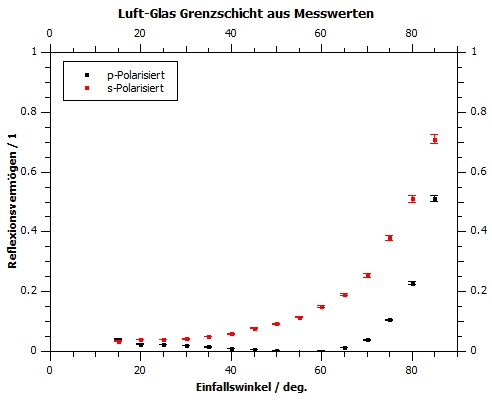
\includegraphics[width=0.6\linewidth]{nudes/LG Mess.jpg}
    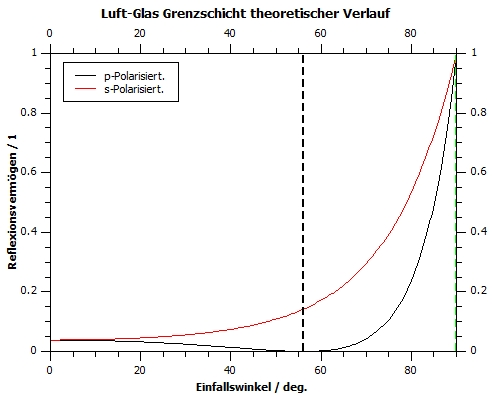
\includegraphics[width=0.6\linewidth]{nudes/LG theor.jpg}
    \caption{Reflexionsvermögen $R$ aus den Messwerten und theoretisch berechnetes Reflexionsvermögen $R$ aus MATLAB für eine Luft-Glas Grenzschicht. \\
    Die Schwarz-Strichlierte Linie kennzeichnet den Brewsterwinkel bei ca. 56°, die Grün-Strichlierte Linie den Grenzwinkel der Totalreflexion bei ca. 90°. }
    \label{fig:reflexionsvermögen LG}
\end{figure}

\begin{figure}[H]
    \centering
    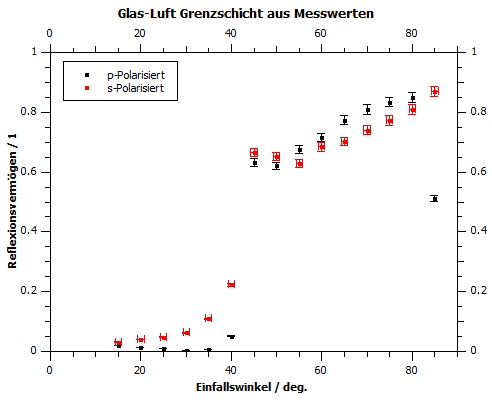
\includegraphics[width=0.6\linewidth]{nudes/GL Mess.jpg}
    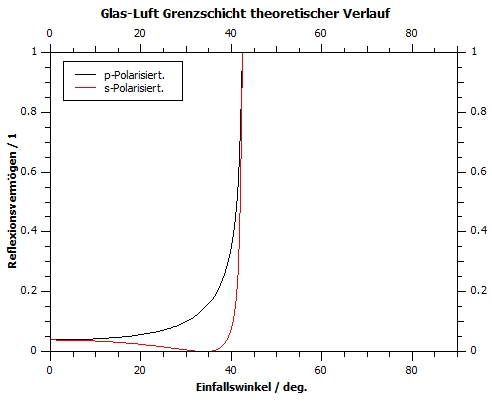
\includegraphics[width=0.6\linewidth]{nudes/GL theor.jpg}
    \caption{Reflexionsvermögen $R$ aus den Messwerten und theoretisch berechnetes Reflexionsvermögen $R$ aus MATLAB für eine Glas-Luft Grenzschicht. \\
    Die Schwarz-Strichlierte Linie kennzeichnet den Brewsterwinkel bei ca. 34°, die Grün-Strichlierte Linie den Grenzwinkel der Totalreflexion bei ca. 42°. }
    \label{fig:reflexionsvermögen GL}
\end{figure}

\noindent
Anmerkung, in den Diagrammen ist die Unsicherheit des Einfallswinkels kaum sichtbar, da diese sehr klein ausfällt. 
\\
\\
Mit den Messwerten aus der Tabelle \ref{tab:brechender Winkel} wird das Brechungsgesetzt (\ref{eq:Snellius}) bewiesen. 
Dazu berechnet man mit den Daten aus Tabelle \ref{fig:reflexionsvermögen LG} den Brechenden Winkel $\varphi_{brech}$. 
Mit bekannten Brechungsindizes $n$ lässt sich der Brechungswinkel $\varphi_{brech}$ berechnen. 
Der Brechungsindex von Luft beträgt dabei $n_L = 1.0$, der Brechungswinkel für Glas beträgt $n_G = 1.488$ \cite{teachcenter2}. 
Eingesetzt in die Formel \ref{eq:Brechender Winkel} kommt man für den Brechenden Winkel auf folgende Werte. 

\begin{table}[H]
    \centering
    \caption{Brechender Winkel $\varphi_{brech}$ berechnet aus den Brechungsindizes $n$ für eine Luft-Glas Grenzfläche. }
    \label{tab:brechender winkel berechnet}
    \begin{tabular}{| l | l | l |}
        \hline
        Nr. & $\varphi_{Ein} \pm 0.7$ / deg.  & $\varphi_{brech} \pm 0.7$ / deg.   \\
        \hline
        1  & 15.0  & 11 $\pm$  2 \\ %10.0168
        2  & 20.0  & 14 $\pm$  2 \\ %13.2884
        3  & 25.0  & 17 $\pm$  2 \\ %16.5001
        4  & 30.0  & 20 $\pm$  2 \\ %19.6347
        5  & 35.0  & 23 $\pm$  2 \\ %22.6728
        6  & 40.0  & 26 $\pm$  3 \\ %25.5933
        7  & 45.0  & 29 $\pm$  3 \\ %28.3728
        8  & 50.0  & 31 $\pm$  3 \\ %30.9851
        9  & 55.0  & 34 $\pm$  3 \\ %33.4017
        10 & 60.0  & 36 $\pm$  4 \\ %35.5918
        11 & 65.0  & 38 $\pm$  4 \\ %37.5229
        12 & 70.0  & 40 $\pm$  4 \\ %39.1619
        13 & 75.0  & 41 $\pm$  4 \\ %40.4771
        14 & 80.0  & 42 $\pm$  5 \\ %41.4398
        15 & 85.0  & 43 $\pm$  5 \\ %42.0274
        \hline
    \end{tabular}
\end{table}

\noindent
Die berechneten Brechenden Winkel werden in einen Diagramm mit den gemessenen Brechenden Winkel dargestellt. 

\begin{figure}[H]
    \centering
    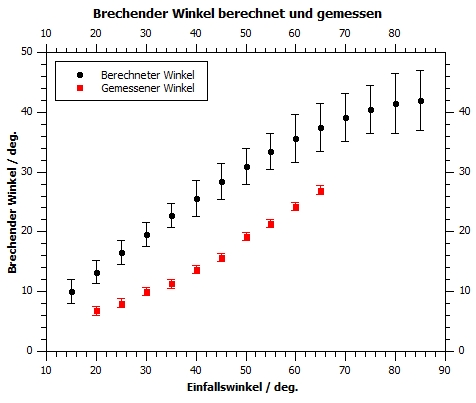
\includegraphics[width=0.6\linewidth]{nudes/brechender winkel.jpg}
    \caption{Brechender Winkel in Abhängigkeit des Einfallswinkels bei einer Luft-Glas Grenzfläche. }
    \label{fig:brechender winkel}
\end{figure}

\noindent
Um nun bei dem Teilversuch Abbe-Refraktometer die Dispersion $n_F-n_C$ zu bestimmen, werden die Messdaten aus der Tabelle \ref{tab:abbe werte} auf die Skalen des Nomogrammes (\ref{fig:nomogramm}) aufgetragen. 
Der Brechungsindex $n_D$ und der Kompensatorwert werden eingezeichnet und geradlinig Verbunden. 
Auf der dazwischenliegenden Skala befindet sich der Wert der Dispersion $n_F-n_C$. 

\begin{figure}[H]
    \centering
    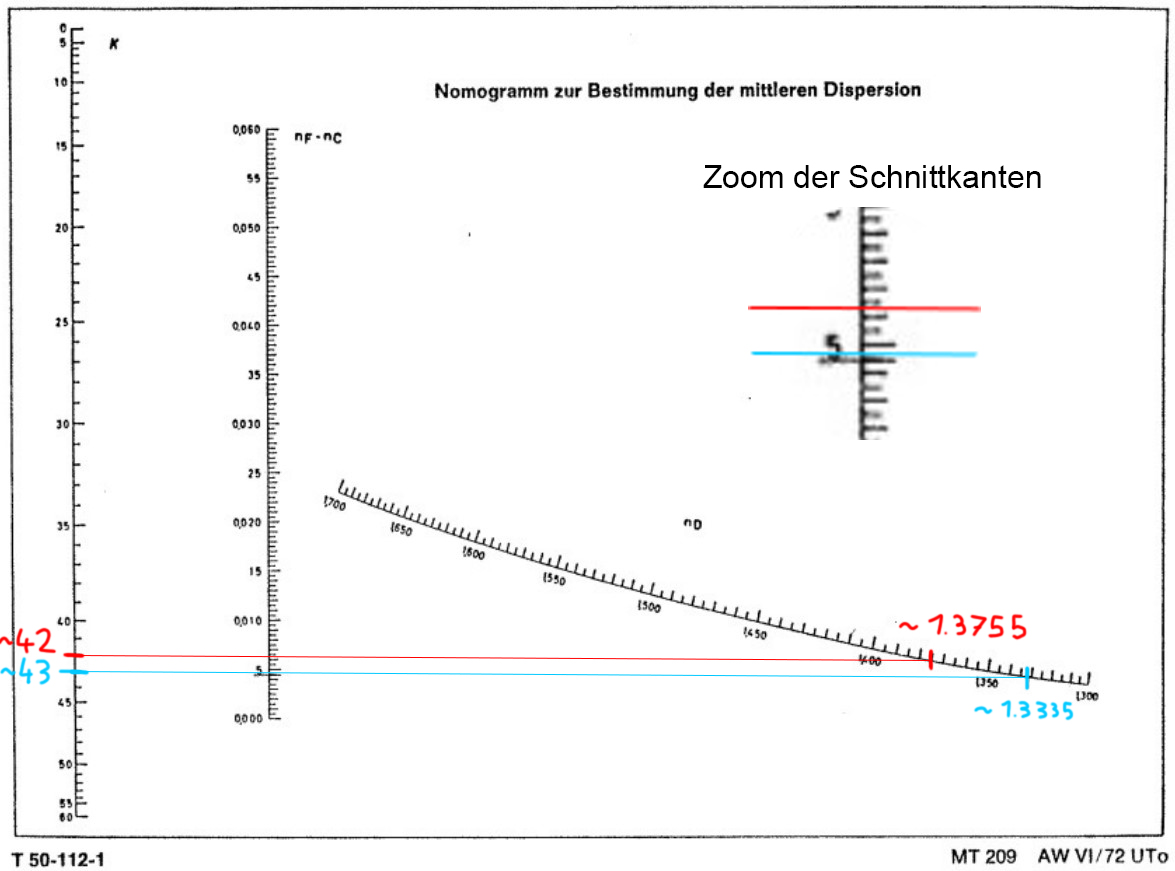
\includegraphics[width=0.6\linewidth]{nudes/nomogramm_auswertung.jpg}
    \caption{Dispersion $n_F-n_C$ des Abbe-Refraktometers auf dem Nomogramm. Die rote Linie entspricht der Zuckerlösung, die blaue der des destilierten Wassers. }
    \label{fig:nomogramm_auswertung}
\end{figure}

\noindent
Wie man hier erkennen kann, beträgt der Wert der Dispersion $n_F-n_C$ für das destilierte Wasser $n_F-n_C = (0.0045 \pm 0.0005)$ sowie für die Zuckerlösung $n_F-n_C = (0.0065 \pm 0.0005)$. 
Die Unsicherheit ist dabei die Ableseunsicherheit des Nomogrammes. 
\\
\\
Somit wurde die Dispersion $n_F-n_C$ bestimmt, jedoch nicht die Menge an gelöstem Zucker in der Flüssigkeit. 
Laut der Tabelle \ref{tab:abbe werte} beträgt die Brix bei der Zuckerlösung $(27.0 \pm 0.5)$ \%.  
Mit diesen Angaben kann man sagen, dass die Messprobe zu $(27.0 \pm 0.5)$ \% Zucker besteht. 


\section{Diskussion} %diskussion der Unsicherheiten und Ergebnisse und evtl. verlgeich mit Literatur ------------------------------
Ein wichtiges Element der Optik ist das Refraktometer. Sei es zum experimentellen Beweis des Brechungsgesetzes oder zur bestimmung der Zuckermenge in einer Lösung. 
\\
In diesem Versuch gilt es das Reflexionsvermögen an der Grenzfläche zweier Medien zu bestimmen. 
Vergleicht man die Ergebnisse mit den theoretisch berechneten Kurven aus MATLAB so sieht man, dass die Ergebnisse den erwartungen gerecht werden. 
Besonders die Messdaten bei der Luft-Glas Grenzfläche sind sehr ähnlich den theoretisch berechneten Kurven. 
Die Ergebnisse liegen im Rahmen der Unsicherheiten, welche sich aus der Nullpunktunsicherheit der Winkelskalen für den Einfallswinkel ergeben. 
Die Unsicherheit des Reflexionsvermögens liegt im Rahmen der theoretisch berechneten Werte. 
\\
\\
Bei dem Glas-Luft übergang weichen die Ergebnisse den theoretischen Kurven etwas ab. Da hier der Laserstrahl zuerst auf eine Luft-Glas Grenzfläche, und dann wieder durch den Prisma auf die Glas-Luft Grenzfläche trifft, 
wird der Transmissionsgrad abgeschwächt. Hier wäre es nötig gewesen, die Refernzintensität dementsprechend zu korrigieren. 
Die Messdaten befinden sich nach dem Grenzwinkel der Totalreflexion nicht mehr im Rahmen der theoretischen Werte. 
Vor diesem Winkel liegen die Werte mit Unsicherheit im Rahmen der theoretischen Werte.  
\\
Es lässt jedoch für den ersten Teil auf eine nahezu fehlerfreie Versuchsdurchführung schließen. 
\\
\\
Im zweiten Teil wird der Brechende Winkel einer Luft-Glas Grenzfläche bestimmt. 
Die gemessenen Werte weichen den berechneten jedoch um ca. 10° ab. Sie liegen auch nicht im Rahmen der Unsicherheit. 
Es lässt darauf schließen, dass bei einem der Werte der Nullpunkt des Lasers und des Prismas nicht richtig getroffen wurde. 
\\
\\
Im dritten Teil wird die Dispersion mit einem Abbe-Refraktometer gemessen. 
Durch Ablesen des Brechungsindex und des Kompensatorwertes lässt sich die Dispersion mithilfe des Nomogrammes bestimmen. 
Die Menge an gelöstem Zucker wird mit der einheit Brix bestimmt. \\
Bei diesem Versuch gibt es keine Vergleichswerte, da der Gehalt der Zuckerlösung nicht bekannt ist. 
 

\section{Zusammenfassung} %klare, übersichtliche vollständige beantwortung der Aufgabenstellung ------------------------------
Hier nocheinmal alle Ergebnisse aus der Auswertung zusammengefasst. 

\begin{figure}[H]
    \centering
    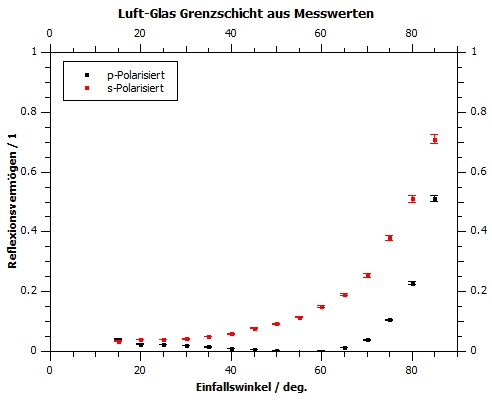
\includegraphics[width=0.6\linewidth]{nudes/LG Mess.jpg}
    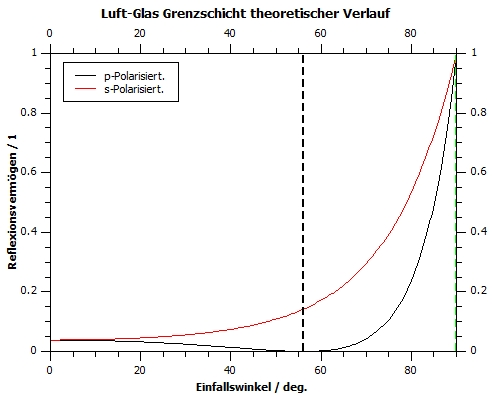
\includegraphics[width=0.6\linewidth]{nudes/LG theor.jpg}
    \caption{Reflexionsvermögen $R$ aus den Messwerten und theoretisch berechnetes Reflexionsvermögen $R$ aus MATLAB für eine Luft-Glas Grenzschicht. \\
    Die Schwarz-Strichlierte Linie kennzeichnet den Brewsterwinkel bei ca. 56°, die Grün-Strichlierte Linie den Grenzwinkel der Totalreflexion bei ca. 90°. }
    \label{fig:zus reflexionsvermögen LG}
\end{figure}

\begin{figure}[H]
    \centering
    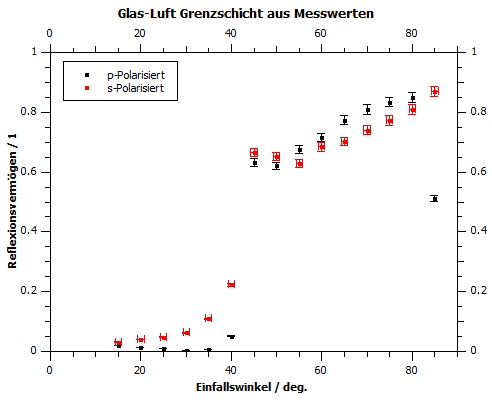
\includegraphics[width=0.6\linewidth]{nudes/GL Mess.jpg}
    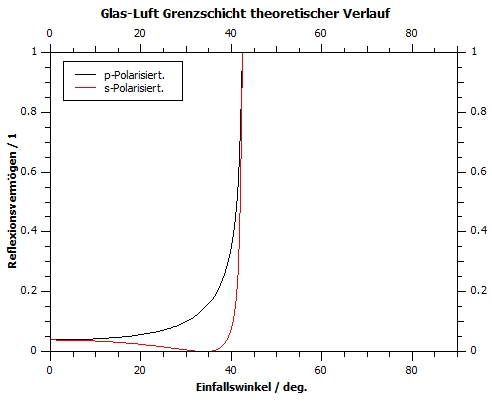
\includegraphics[width=0.6\linewidth]{nudes/GL theor.jpg}
    \caption{Reflexionsvermögen $R$ aus den Messwerten und theoretisch berechnetes Reflexionsvermögen $R$ aus MATLAB für eine Glas-Luft Grenzschicht. \\
    Die Schwarz-Strichlierte Linie kennzeichnet den Brewsterwinkel bei ca. 34°, die Grün-Strichlierte Linie den Grenzwinkel der Totalreflexion bei ca. 42°. }
    \label{fig:zus reflexionsvermögen GL}
\end{figure}

\begin{figure}[H]
    \centering
    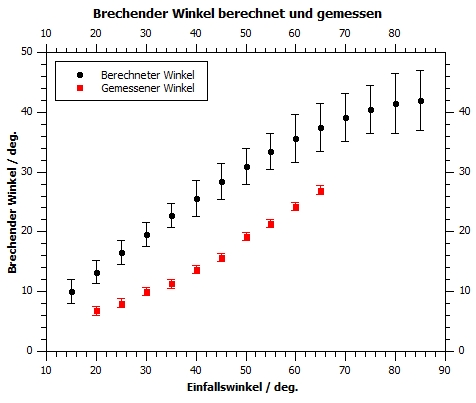
\includegraphics[width=0.6\linewidth]{nudes/brechender winkel.jpg}
    \caption{Brechender Winkel in Abhängigkeit des Einfallswinkels bei einer Luft-Glas Grenzfläche. }
    \label{fig:zus brechender winkel}
\end{figure}

\begin{itemize}
    \item Dispersion destilliertes Wasser $n_F-n_C = 0.0045 \pm 0.0005$
    \item Dispersion Zuckerlösung $n_F-n_C = 0.0065 \pm 0.0005$
    \item Zuckergehalt in \% = $(27.0 \pm 0.5) \%$
\end{itemize}



\section{Anhang}

\begin{verbatim}
% Berechnung der Reflexion an einer Grenzfläche zwischen zwei Medien mit n1 und n2
% Lichteinfall von Seite 1 / n1

%default für Plots
set(0,'defaultaxesfontname','arial','defaultaxesfontsize',12,'defaultlinelinewidth',2);

%Brechzahlen
n1=1.488;     %Glas
n2=1.0;       %Luft             

%Luft-Glas Grenzfläche
aein1=linspace(0,90,200).'*pi/180; % Einfallswinkel alpha_1, 200 Werte (0-90°) in Radiant
b1=asin(sin(aein1)*n1/n2); % Brechungswinkel beta_1, berechnet aus dem Brechungsgesetz
rho_p1=(n2*cos(aein1)-n1*cos(b1))./(n2*cos(aein1)+n1*cos(b1)); % Reflexionskoeff. für p-Pol.
rho_s1=(n1*cos(aein1)-n2*cos(b1))./(n1*cos(aein1)+n2*cos(b1)); % Reflexionskoeff. für s-Pol.

%Glas-Luft Grenzfläche
aein2=linspace(0,90,200).'*pi/180; % Einfallswinkel alpha_2, 200 Werte (0-90°) in Radiant
b2=asin(sin(aein2)*n2/n1); % Brechungswinkel beta_2, berechnet aus dem Brechungsgesetz
rho_p2=(n2*cos(aein2)-n1*cos(b2))./(n2*cos(aein2)+n1*cos(b2)); % Reflexionskoeff. für p-Pol.
rho_s2=(n1*cos(aein2)-n2*cos(b2))./(n1*cos(aein2)+n2*cos(b2)); % Reflexionskoeff. für s-Pol.


R_s1=abs(rho_s1.^2); % Reflexionsvermögen für s-Pol. für Luft-Glas Grenzfläche
R_p1=abs(rho_p1.^2); % Reflexionsvermögen für p-Pol. für Luft-Glas Grenzfläche
R_s2=abs(rho_s2.^2); % Reflexionsvermögen für p-Pol. für Luft-Glas Grenzfläche
R_p2=abs(rho_p2.^2); % Reflexionsvermögen für p-Pol. für Luft-Glas Grenzfläche


% Plotten der Funktion
figure(1);
clf();
plot(aein1*180/pi,[R_s1, R_p1]);  %Plot der Funktionen für Luft-Glas
hold on;
plot(aein2*180/pi,[R_s2, R_p2]); %Plot der Funktionen für Glas Luft
title('Eisner, Waldl');
xlabel('Einfallswinkel / °');
ylabel('Reflexionsvermögen / 1');
legend('s-Pol_GL','p-Pol_GL', 's-Pol_LG', 'p-Pol_LG', 'location','northwest');
ylim([0,1.05]);
xlim([0,90]);
hold on;

%Schreiben der Daten in eine .csv für QtiPlot
dlmwrite('Reflexionswerte-Luft-Glas.csv', [aein1*180/pi, R_s1, R_p1],'\t');
dlmwrite('Reflexionswerte-Glas-Luft.csv', [aein2*180/pi, R_s2, R_p2],'\t');
\end{verbatim}

\printbibliography[heading=bibintoc]

\end{document}
